% T12 C/D, chapitre 2 : Probabilités. Source : le livre « Terminales scientifiques » (Proba/Lesona, Proba/Fiche, Proba/Exo).
% Les exercices tirés d’autres ouvrages ne sont pas repris (décision du 2 novembre 2026).

\TCDLessonStyleOn
\chapter{Probabilit\'e}
\newcommand{\card}[1]{\text{Card }#1}
\newcommand{\A}[2]{A_{#1}^{#2}}
\newcommand{\C}[2]{C_{#1}^{#2}}
      \section{D\'enombrement}
            %
            \begin{defi}[Cardinal d'un ensemble fini]
\index{Cardinal}
            On appelle \emph{cardinal} d'un ensemble fini le nombre de ses \'el\'ements.
            Si $X$ est un ensemble alors nous noterons par $Card(X)$ le cardinal de $X$.
            Si on se place dans un ensemble $E$ et si $A$ est un sous-ensemble de $E$, alors on note par $\bar{A}$ le compl\'ementaire de $A$ dans $E$, c'est-\`a-dire l'ensemble des \'el\'ements de $E$ qui ne sont pas dans $A$. 
            \end{defi}
            %
            \begin{prp}
            Soient $A$ et $B$ deux ensembles finis. On a alors :
            \begin{itemize}
                  \item Si $A$ et $B$ sont deux ensembles disjoints, alors $Card(A \cup B) = Card(A) + Card(B)$.
                  \item $Card(A \cup B) = Card(A) + Card(B) - Card(A \cap B)$.
                  \item Si $\bar{A}$ d\'esigne le compl\'ementaire de $A$ dans $E$, alors $Card(\bar{A}) = Card(E) - Card(A)$.
            \end{itemize}
            \end{prp}
            %
            Soient $E$ et $F$ deux ensembles finis non-vides \`a $p$ et $n$ \'el\'ements respectivement.
            Notons par $e_1,\ e_2,\ \ldots\ ,\ e_p$ les \'el\'ements de $E$ 
            et par  $f_1,\ f_2,\ \ldots\ ,\ f_n$ les \'el\'ements de $F$. 
            %
            \subsection{Nombre d'applications de $E$ vers $F$}
            Si $\varphi : E \rightarrow F $ 
            est une application, alors :
            \begin{itemize}
                  \item il y a $n$ possibilit\'es pour $\varphi(e_1)$,
                  \item il y a $n$ possibilit\'es pour $\varphi(e_2)$,
                  \item et ainsi de suite,
                  \item il y a $n$ possibilit\'es pour $\varphi(e_p)$.
            \end{itemize}
            Ainsi, il y a exactement \propbox{$n^p$} applications possibles de $E$ dans $F$.
            %
            \begin{figure}[h!]
            \centering
                  \begin{tikzpicture}[line cap=round,line join=round,>=triangle 45,x=1.0cm,y=1.0cm]
                  \clip(-2.7,0.26) rectangle (5.44,5.32);
                  \draw [rotate around={89.01:(-1.56,2.7)}] (-1.56,2.7) ellipse (1.38cm and 0.74cm);
                  \draw [rotate around={89.16:(4.25,2.72)}] (4.25,2.72) ellipse (2.27cm and 1cm);
                  \draw [->] (-1.82,3.63) -- (4.64,3.75);
                  \draw [->] (-1.37,1.57) -- (4.64,3.75);
                  \draw [->] (-1.42,3) -- (4.43,2.6);
                  \draw [->] (-1.81,2.24) -- (4.44,1.05);
                  \begin{scriptsize}
                  \fill [color=black] (-1.82,3.63) circle (1.5pt);
                  \draw[color=black] (-1.67,3.77) node {$e_1$};
                  \fill [color=black] (-1.42,3) circle (1.5pt);
                  \draw[color=black] (-1.27,3.13) node {$e_2$};
                  \fill [color=black] (-1.81,2.24) circle (1.5pt);
                  \draw[color=black] (-1.64,2.37) node {$e_3$};
                  \fill [color=black] (-1.37,1.57) circle (1.5pt);
                  \draw[color=black] (-1.25,1.75) node {$e_4$};
                  \fill [color=black] (3.98,4.42) circle (1.5pt);
                  \draw[color=black] (4.11,4.56) node {$f_1$};
                  \fill [color=black] (4.64,3.75) circle (1.5pt);
                  \draw[color=black] (4.79,3.88) node {$f_2$};
                  \fill [color=black] (3.66,3.09) circle (1.5pt);
                  \draw[color=black] (3.8,3.23) node {$f_3$};
                  \fill [color=black] (4.43,2.6) circle (1.5pt);
                  \draw[color=black] (4.46,2.79) node {$f_4$};
                  \fill [color=black] (3.89,1.71) circle (1.5pt);
                  \draw[color=black] (4.03,1.85) node {$f_5$};
                  \fill [color=black] (4.44,1.05) circle (1.5pt);
                  \draw[color=black] (4.58,1.19) node {$f_6$};
                  \end{scriptsize}
                  \end{tikzpicture}
                  \caption{
                           Exemple d'application d'un ensemble $E$ de $4$ \'el\'ements 
                           vers un ensemble $F$ de $6$ \'el\'ements.
                           }
            \end{figure}
            \subsection{Arrangements dans un ensemble fini}
\index{Arrangement}
                  \begin{defi}
                        Soient $E$ un ensemble fini \`a $n$ \'el\'ements et $p$ un nombre entier inf\'erieur ou \'egal \`a $n$.
                        On appelle \emph{arrangement de $p$ \'el\'ements de $E$}, et on note 
                        \defbox{$\displaystyle{\Arr{n}{p}}$}, le nombre de mani\`eres de choisir $p$ \'el\'ements de $E$ en tenant compte de l'ordre
                        (c'est-\`a-dire le nombre de listes de $p$ \'el\'ements distincts de $E$).
                  \end{defi}
                  %
                  	\begin{prop}
                  			\propbox{
                 				\[
                  					\Arr{n}{p} = \frac{n!}{(n-p)!}
                  				\]}
                  	\end{prop}
						%
						\begin{ex}
							Consid\'erons quatre personnes num\'erot\'ees de 1 \`a 4
							ainsi que six chaises marqu\'ees par les lettres a, b, \ldots, f.
							%
							On veut conna\^itre le nombre de fa\c{c}ons dont ces quatre personnes
							peuvent s'asseoir sur les six chaises ;
							on ne tol\`ere pas que deux personnes s'assoient sur la m\^eme chaise.
							\begin{valiny}
								Pour cel\`a, posons	$E = \{ 1 ,\ 2,\ 3,\ 4 \}$ et 
															$F = \{ a,\ b,\ c,\ d,\ e,\ f \}$.
								\begin{itemize}
									\item La personne num\'ero $1$ a $6$ choix possibles et, apr\`es qu'elle a pris sa place,
									\item la personne num\'ero $2$ a $5$ choix possibles,
									\item la personne num\'ero $3$ a $4$ choix possibles,
									\item la personne num\'ero $4$ a $3$ choix possibles.
								\end{itemize}
								En tout, cel\`a fait $6\times 5 \times 4 \times 3 = 360$ possibilit\'es.
								%
									Ce nombre peut aussi se calculer par la formule
								$\A{6}{4} 
									= \frac{6!}{2!} 
									= \frac{6\times 5 \times 4 \times \cdots \times 3 \times 2 \times 1}{2 \times 1}
									= 360
								$.
							\end{valiny}
						\end{ex}
					%
            \subsection{Permutation dans un ensemble fini}
\index{Permutation}
                  Si on prend $E = F$ dans le cas pr\'ec\'edent, alors on se retrouve avec ce que l'on appelle
                  \emph{permutation de $E$}.
                  Le nombre de permutations d'un ensemble \`a $n$ \'el\'ements est $n!$.
                  \begin{ex}
                        Consid\'erons une course avec six participants. 
                        A l'issue de la course, on suppose qu'il n'y a pas d'ex aequo.
                        On veut d\'eterminer le nombre de possibilit\'es de r\'esultats pour une telle course.
                     \begin{valiny}
                        \begin{itemize}
                              \item Il y a $6$ possibilit\'es pour la premi\`ere place,
                              \item il y a $5$ possibilit\'es pour la seconde place,
                              \item $\vdots$ 
                              \item il y a $1$ possibilit\'e pour la derni\`ere place.
                        \end{itemize}
                        Ainsi, il y a $6 \times 5 \times \cdots \times 1$ issues possibles.
                        Ce nombre est $6! = 720$.
                     \end{valiny}
                  \end{ex}
				\subsection{Combinaison dans un ensemble fini}
\index{Combinaison}
					\begin{defi}
						Soient $E$ un ensemble fini \`a $n$ \'el\'ements et $p$ un nombre entier naturel inf\'erieur ou \'egal \`a $n$.
						On appelle \emph{nombre de combinaisons de $p$ \'el\'ements de $E$} le nombre, not\'e 
						\defbox{$\displaystyle{\Comb{n}{p}}$},
							de mani\`eres de choisir $p$ \'el\'ements de $E$.
					\end{defi}
					%
                  	\begin{prop}~\\[-1\baselineskip]
								\propbox{
									\[
										\Comb{n}{p} = \frac{n!}{p!\;(n-p)!}
									\]
								}
 						\end{prop}
 					%
 					\begin{ex}
	 						On dispose d'un d\'e cubique \`a six faces, num\'erot\'ees de $1$ \`a $6$.
 						On veut colorer deux des faces de ce d\'e, de mani\`ere \`a cacher les num\'eros y figurant.
 						De combien de mani\`eres peut-on le faire\,?
 						\begin{valiny}
	 						Il suffit de << choisir >> deux faces parmi les 6.
 							Il y a, par cons\'equent, 
 							$\Comb{6}{2} = \frac{6!}{2! \; (6-2)!} = 15$ fa\c{c}ons de colorer deux faces d'un d\'e cubique.
 						\end{valiny}
 					\end{ex}
%
      \section{Notion de probabilit\'e}
            \begin{defi}[\'Epreuve ou exp\'erience al\'eatoire]
\index{Epreuve@\'Epreuve}
\index{Experience aleatoire@Exp\'erience al\'eatoire}
                  Une \emph{exp\'erience al\'eatoire} est une exp\'erience renouvelable
                  dont le r\'esultat ne peut \^etre pr\'evu, et qui, renouvel\'ee dans des conditions identiques
                  ne donne pas forc\'ement le m\^eme r\'esultat \`a chaque renouvellement.
                  \begin{ex}
                        \begin{itemize}
                              \item Lancement d'un d\'e,
                              \item tirage de boules dans une urne.
                        \end{itemize}
                  \end{ex}
            \end{defi}
            %
            \begin{defi}[Univers, \'eventualit\'es, \'ev\`enement]
\index{Univers des eventualite@Univers des \'eventualit\'es}
                  L'ensemble de tous les r\'esultats possibles est appel\'e \emph{univers des \'eventualit\'es}.
                  L'univers est souvent not\'e $\Omega$.
                  %
                  Les \'el\'ements de $\Omega$ sont appel\'es \emph{\'eventualit\'es}.
\index{Eventualite@\'Eventualit\'e}
                  On appelle \emph{\'ev\`enement} tout ensemble d'\'eventualit\'es, c'est-\`a-dire toute partie de $\Omega$.
\index{Evenements@\'Ev\`enements}
                  Si $A$ est un \'ev\`enement, on note par $\bar{A}$ le compl\'ementaire de $A$ dans $\Omega$,
                  $\bar{A}$ est appel\'e l'\emph{\'ev\`enement contraire de $A$}.
\index{Evenements@\'Ev\`enements!contraires}
                  Deux \'ev\`enements $A$ et $B$ sont dits \emph{incompatibles} si $A\cap B = \emptyset$.
\index{Evenements@\'Ev\`enements!incompatibles}
                  \begin{ex}
                        Consid\'erons les \'epreuves suivantes :
                        \begin{enumerate}
                              \item Lancer d'un d\'e \`a six faces.
                                    L'univers des possibilit\'es est 
                                    $\Omega = \{ 1,\ 2,\ 3,\ 4,\ 5,\ 6 \}$.
                              \item Lancer de deux pi\`eces de monnaie distinctes.
                                    L'univers des possibilit\'es est
                                    \[
                                      \Omega = \left\{
                                        \begin{array}{cc}
                                          (\text{Pile},\text{Pile}), & (\text{Pile},\text{Face}), \\
                                          (\text{Face},\text{Pile}), & (\text{Face},\text{Face})
                                        \end{array}
                                      \right\}.
                                    \]
                        \end{enumerate}
                  \end{ex}
                  %
                  \begin{ex}
                        On lance un d\'e cubique dont les six faces sont num\'erot\'ees par les nombres 
                        1, 2, 3, 4, 5 et 6.
                        
                        \begin{enumerate}
                              \item L'univers est : $\Omega = \{1,\ 2,\ 3,\ 4,\ 5,\ 6 \}$.
                              \item Consid\'erons les \'ev\`enements : 
                                    \begin{align*}
                                    A &: \text{<< Obtenir un nombre pair >>} \\
                                    B &: \text{<< Obtenir un nombre inf\'erieur ou \'egal \`a 3 >>} .
                                    \end{align*}
                                    On a donc $A = \{ 2,\ 4,\ 6 \}$ et $B = \{ 1,\ 2,\ 3 \}$.
                              \item L'\'ev\`enement << $A$ ou $B$ >> est $A \cup B = \{ 1,\ 2,\ 3,\ 4,\ 6 \}$.
                              \item L'\'ev\`enement << $A$ et $B$ >> est $A \cap B = \{ 2 \}$, 
                                    c'est un \emph{\'ev\`enement \'el\'ementaire}.
                              \item $\bar{A} = \{ 1,\ 3,\ 5 \}$ et $\bar{B} = \{ 4,\ 5,\ 6 \} $.
                              \item $A$ et $\bar{A}$ sont incompatibles.
                                    En fait, quel que soit l'\'ev\`enement $X$, $X$ et $\bar{X}$ sont toujours incompatibles.
\index{Evenements@\'Ev\`enements!elementaires@\'el\'ementaires}
                        \end{enumerate}
                  \end{ex}
            \end{defi}
      Consid\'erons un univers fini $\Omega = \{ \omega_1,\ \omega_2,\ \ldots ,\omega_n \}$.
      \begin{defi}[Probabilit\'e]
\index{Probabilite@Probabilit\'e}
            On appelle \emph{probabilit\'e} sur $\Omega$ toute application 
            de l'ensemble des \'ev\`enements dans $[0 ; 1]$ telle que : 
            \begin{itemize}
                  \item la somme des probabilit\'es des \'ev\`enements \'el\'ementaires est \'egale \`a $1$,
                  \item la probabilit\'e d'un \'ev\`enement est \'egale \`a la somme des probabilit\'es
                        des \'ev\`enements \'el\'ementaires qui le constituent.
            \end{itemize}
      \end{defi}
      %
      \begin{prop}
            Soient $\Omega$ l'univers et $A$ et $B$ deux \'ev\`enements.
            Soit $P$ une probabilit\'e sur $\Omega$. On a :
            \begin{itemize}
                  \item $P(\emptyset ) = 0$ et $P(\Omega ) = 1$,
                  \item $P(\bar{A}) = 1 - P(A)$,
                  \item $P(A\cup B) = P(A) + P(B) - P(A\cap B)$.
                        Si $A$ et $B$ sont incompatibles, alors $P(A\cup B) = P(A) + P(B)$.
                  \item Si $A\subseteq B$ alors $P(A) \leq P(B)$.
            \end{itemize}
      \end{prop}
      %
      \subsection*{Le cas \'equiprobable}
\index{Equiprobabile@\'Equiprobable}
            On dit qu'il y a \emph{\'equiprobabilit\'e} lorsque tous les \'ev\`enements 
            \'el\'ementaires ont la m\^eme probabilit\'e.
            Dans le cas \'equiprobable, si $\omega$ est un \'ev\`enement \'el\'ementaire, alors
                  $P(\{\omega\}) = \frac{1}{\card{\Omega}}$.
            Si $A$ est un \'ev\`enement quelconque, alors 
            \thmbox{
                  $$P(A) = \frac{\card{A}}{\card{\Omega}} 
                        = \frac{\text{Nombre de cas favorables}}{\text{Nombre de cas possibles}}.$$}
            \begin{exe}\label{exe:proba-cours-1}
                        On consid\`ere un lancer de d\'e non truqu\'e.
                        La probabilit\'e de chaque \'ev\`enement \'el\'ementaire est \'egale \`a $\frac{1}{6}$.
                        Soient les \'ev\`enements : 
                              \begin{enumerate}
                                    \item A : << Obtenir un nombre pair. >>
                                    \item B : << Obtenir un nombre inf\'erieur ou \'egal \`a 3. >>
                              \end{enumerate}
                        Calculer les probabilit\'es : $P(A)$, $P(B)$, $P(A\cap B)$ et $P(A \cup B)$.
            \end{exe}
            %
            \begin{exe}\label{exe:proba-cours-2}
                        On consid\`ere maintenant un d\'e truqu\'e de sorte que 
                              la probabilit\'e d'obtenir $6$ soit deux fois la probabilit\'e d'obtenir $1$,
                              la probabilit\'e d'obtenir $1$ \'etant la m\^eme que celle d'obtenir $2$, $3$, $4$ ou $5$.
                              \begin{enumerate}
                                    \item Calculer la probabilit\'e de chaque \'ev\`enement \'el\'ementaire.
                                    \item Calculer la probabilit\'e des \'ev\`enements :
                                          \begin{enumerate}
                                                \item A : << Obtenir un nombre pair. >>
                                                \item B : << Obtenir un nombre inf\'erieur ou \'egal \`a 3. >>
                                          \end{enumerate}
                              \end{enumerate}
            \end{exe}
            %
            \begin{exe}\label{exe:proba-cours-3}
                        Dans une urne contenant 10 boules num\'erot\'ees de 0 \`a 9,
                        on tire successivement et avec remise 3 boules.
                        \begin{enumerate}
                              \item Calculer le nombre de tirages possible.
                              \item Calculer le nombre de tirages telle que 
                                    la premi\`ere boule ne soit pas celle num\'erot\'ee 0.
                              \item Calculer la probabilit\'e que les num\'eros tir\'es dans l'ordre
                                    forment un nombre de trois chiffres
                                    (c'est-\`a-dire ne commen\c{c}ant pas par 0).
                        \end{enumerate}
                        (On admet que toutes les boules ont la m\^eme probabilit\'e d'\^etre tir\'ee.)
            \end{exe}
            %
            \begin{exe}\label{exe:proba-cours-4}
                        On consid\`ere un urne contenant 26 boules,
                        chacune marqu\'ee d'une lettre de l'alphabet (fran\c{c}aise) diff\'erente.
                        On tire successivement et sans remise cinq boules de l'urne.
                        \begin{enumerate}
                              \item Calculer le nombre de tirages possible.
                              \item Calculer la probabilit\'e d'obtenir les cinq lettres `M A T H S' dans cet ordre.
                              \item Calculer la probabilit\'e d'obtenir les cinq lettres `A H M S T',
                                    pas n\'ecessairement dans cet ordre.
                              \item Calculer la probabilit\'e d'obtenir cinq voyelles (on compte six voyelles : A, E, I, O, U et Y).
                        \end{enumerate}
            \end{exe}
            %
            \begin{exe}\label{exe:proba-cours-5}
                        Dans un jeu de 52 cartes, on tire 13 cartes simultan\'ement.
                        Calculer la probabilit\'e d'avoir : 
                        \begin{enumerate}
                              \item Exactement un as,
                              \item exactement deux as,
                              \item exactement trois as,
                              \item exactement quatre as,
                              \item exactement cinq as,
                              \item uniquement des tr\`efles.
                        \end{enumerate}
            \end{exe}
      %
      %
      \section{Probabilit\'e conditionnelle}
\index{Probabilite@Probabilit\'e!conditionnelle}
            \subsection{Probabilit\'e conditionnelle}
            Consid\'erons un univers $\Omega$ et soient $A$ et $B$ deux \'ev\`enements.
            Soit $P$ une probabilit\'e.
            On suppose que $P(B) \neq 0$.
            La \emph{probabilit\'e de $A$ sachant $B$} est 
                  \defbox{
                              \[
                                    P(A|B) = \frac{P(A\cap B)}{P(B)}.
                              \]
                         }
            \begin{ex}
                  Une urne contient neuf boules indiscernables au toucher.
                  Les boules sont num\'erot\'ees de 1 \`a 9.
                  On tire une boule au hasard.
                  Soient les \'ev\`enements : 
                  \begin{enumerate}
                        \item A : << Le num\'ero tir\'e est pair. >>
                        \item B : << Le num\'ero tir\'e est un multiple de 3. >>
                  \end{enumerate}
                  
                  On a $ \Omega = \{ 1,\ 2,\ 3,\ 4,\ 5,\ 6,\ 7,\ 8,\ 9 \}$,
                       $ A = \{ 2,\ 4,\ 6,\ 8 \}$ et
                       $ B = \{ 3,\ 6,\ 9 \}$.
                  Il suit que $A \cap B = \{ 6 \}$.
                  Ainsi, $P(A) = \frac{4}{9}$, $P(B) = \frac{3}{9} = \frac{1}{3}$ et $P(A\cap B) = \frac{1}{9}$.
                  
                  Supposons qu'on sait qu'on a obtenu un multiple de 3.
                  Quelle est alors la probabilit\'e pour que ce soit un num\'ero pair\,?
                  
                  Il suffit de calculer 
                        \[
                        P(A|B) = \frac{P(A\cap B)}{P(B)} = \frac{\frac{1}{9}}{\frac{1}{3}} = \frac{1}{3}.
                        \]
            \end{ex}
            \smallnota{
            La probabilit\'e de $A$ sachant $B$ est aussi parfois not\'e $P_B (A)$.
            }
            %
            \begin{exe}\label{exe:proba-cours-6}
                  On vous propose de jouer \`a un jeu.
                  On pose devant vous cinq paniers clos ; 
                  l'un d'eux contient une pi\`ece de monnaie tandis que
                  les quatre autre sont vides.
                  %
                  Votre objectif est de trouver la pi\`ece de monnaie.
                  
                  Vous avez le droit de choisir un panier, 
                  vous n'avez aucun moyen de d\'ecider d'une mani\`ere rationnelle quel panier choisir.
                  %
                  Apr\`es que vous avez fait votre choix, l'organisateur, qui sait o\`u se trouve la pi\`ece,
                  ouvre volontairement trois des quatre autres paniers, choisis vides ;
                  votre panier reste clos.
                  %
                  Il reste donc deux paniers clos : le v\^otre et un autre.
                  
                  On vous demande ensuite votre d\'ecision finale : 
                        allez-vous changer votre choix et miser sur l'autre panier ou
                        allez-vous garder votre choix initial\,?
                        
                        \paragraph{Illustration}
                              Supposons que les cinq paniers sont num\'erot\'es de 1 \`a 5.
                              
                                    \begin{tikzpicture}[scale=2]
                                    \foreach \x in {1,2,3,4,5}
                                          \draw[pattern=checkerboard,pattern color=loko2] 
                                                (\x-.3,.3) -- (\x+.3,.3) 
                                                {[rounded corners = 10] -- (\x+.3,-.3) -- (\x-.3,-.3) -- (\x-.3,.3)}
                                                (\x,0) node[fill=white]{\x}
 ;
                                    \end{tikzpicture}
                                    
                              Disons que vous avez choisi le panier 1.
                              
                                    \begin{tikzpicture}[scale=2]
                                    \foreach \x in {1,2,3,4,5}
                                          \draw[pattern=checkerboard,pattern color=loko2] 
                                                (\x-.3,.3) -- (\x+.3,.3) 
                                                {[rounded corners = 10] -- (\x+.3,-.3) -- (\x-.3,-.3) -- (\x-.3,.3)}
                                                (\x,0) node[fill=white]{\x}
 ;
                                          \draw[color=loko1] (1,0) circle (.5);
                                    \end{tikzpicture}
                                    
                              On ouvre ensuite les paniers 2, 3 et 4 qui s'av\`erent \^etre vides.
                              
                                    \begin{tikzpicture}[scale=2]
                                    \foreach \x in {1,2,3,4,5}
                                          \draw[pattern=checkerboard,pattern color=loko2] 
                                                (\x-.3,.3) -- (\x+.3,.3) 
                                                {[rounded corners = 10] -- (\x+.3,-.3) -- (\x-.3,-.3) -- (\x-.3,.3)}
                                                (\x,0) node[fill=white]{\x}
 ;
                                          \draw[color=loko1] (1,0) circle (.5);
                                    \foreach \x in {2,3,4}
                                          \draw[line width=5,color=loko1,opacity=.5] 
                                                (\x+.3,.3) -- (\x-.3,-.3) 
                                                (\x+.3,-.3) -- (\x-.3,.3)
 ;
                                    \end{tikzpicture}
                                    
                              Il reste alors deux paniers clos : les num\'eros 1 et 5.
                              
                                    \begin{tikzpicture}[scale=2]
                                    \foreach \x in {1,5}
                                          \draw[pattern=checkerboard,pattern color=loko2] 
                                                (\x-.3,.3) -- (\x+.3,.3) 
                                                {[rounded corners = 10] -- (\x+.3,-.3) -- (\x-.3,-.3) -- (\x-.3,.3)}
                                                (\x,0) node[fill=white]{\x}
 ;
                                    \foreach \x in {1,5}
                                          \draw[opacity=.5] 
                                                (\x,0) node[fill=white]{{\fontsize{40}{40} \selectfont\,?} }
 ;
                                    \end{tikzpicture}
                                    
                              Allez-vous changer votre choix et miser sur le num\'ero 5
                              ou allez-vous rester ferme \`a votre intuition initiale et garder le num\'ero 1\,?
            \end{exe}
            %
            \subsection{\'Ev\`enements ind\'ependants}
\index{Evenements@\'Ev\`enements!independants@ind\'ependants}
            Deux \'ev\`enements $A$ et $B$ sont dits \emph{ind\'ependants} si 
                        \defbox{$$P(A\cap B) = P(A) \cdot P(B).$$}
            Si deux \'ev\`enements $A$ et $B$ sont ind\'ependants, on a :
                  \begin{displaymath}
                        P(A|B) = \frac{P(A\cap B)}{P(B)} = \frac{P(A) \cdot P(B)}{P(B)} = P(A).
                  \end{displaymath}
            %
            \begin{ex}
                  On dispose d'une pi\`ece de monnaie non truqu\'ee.
                  On proc\`ede \`a deux lancers successifs.
                  Calculer la probabilit\'e d'obtenir pile puis face.
                  \begin{valiny}
                        Soient les deux \'ev\`enements : 
                              \begin{itemize}
                                    \item A : << Le premier lancer donne pile. >>
                                    \item B : << Le second lancer donne face. >>
                              \end{itemize}
                        Ces deux \'ev\`enements sont ind\'ependants --- 
                        le r\'esultat de la premi\`ere n'affecte pas celui de la seconde.
                        On cherche $P(A\cap B)$.
                        On sait que 
                        $P(A\cap B) = P(A) \cdot P(B) = \frac{1}{2} \cdot \frac{1}{2} = \frac{1}{4}$.
                  \end{valiny}
            \end{ex}
            %
	\section{\'Epreuve de Bernoulli et distribution binomiale}
                  \subsection{\'Epreuve de Bernoulli}
\index{Bernoulli}
                        Dans certaines exp\'eriences al\'eatoires, 
                        on s'interesse \`a la r\'ealisation d'un \'ev\`enement.
                        On parlera de << \emph{succ\`es} >> si l'\'ev\`enement se r\'ealise
\index{succes@succ\`es}
                        et d'<<~\emph{\'echec} >> sinon.
\index{echec@\'echec}
                        Ce type d'exp\'erience est appel\'e \emph{\'epreuve de Bernoulli}.
\index{Bernoulli!epreuve de@\'epreuve de}
                        On appelle << \emph{sch\'ema de Bernoulli} >> une succession d'\'epreuves de ce type, identiques et ind\'ependantes.
\index{Bernoulli!schema de@sch\'ema de}
                        %
                        \begin{ex}
                              On lance $n$ fois une pi\`ece,
                              on consid\`ere comme un succ\`es le fait d'obtenir pile
                              (et donc comme \'echec si on obtient face).
                              
                              Le tirage successif et avec remise d'une boule dans une urne.
                              Le succ\`es peut \^etre d\'efini comme l'obtention d'un certain type de boule.
                        \end{ex}
                  \subsection{Distribution binomiale}
                        Consid\'erons un sch\'ema de Bernoulli qui 
                        consiste \`a la succession de $n$ \'epreuves identiques et ind\'ependantes.
                        Soient $p$ la probabilit\'e d'un succ\`es et $q ( = 1-p)$ la probabilit\'e d'un \'echec.
                        Soit $k$ un nombre entier naturel compris entre $0$ et $n$.
                        On veut conna\^itre la probabilit\'e d'avoir $k$ succ\`es au cours des $n$ lancers.
                        
                        La probabilit\'e d'avoir 
                        uniquement des succ\`es au cours des $k$ premiers lancers
                        et uniquement des \'echecs au cours des $n-k$ autres lancers est : 
                              \begin{displaymath}
                                    p^k \cdot (1-p)^{n-k}.
                              \end{displaymath}
                        Il y a $\C{n}{k}$ mani\`eres de r\'epartir les $k$ succ\`es parmi les $n$ \'epreuves.
                        La probabilit\'e d'obtenir $k$ succ\`es est donc 
                                    \thmbox{$$ \C{n}{k}\ p^k \cdot (1-p)^{n-k}. $$}
                        %
                        \begin{ex}
                              On jette 100 fois une pi\`ece de monnaie truqu\'ee de mani\`ere \`a ce que 
                              la probabilit\'e d'obtenir face soit trois fois celle d'obtenir pile. \newline
                              Calculer la probabilit\'e d'avoir 25 fois pile.
                              %
                              \begin{valiny}
                                    Soient $p$ la probabilit\'e d'obtenir pile et $q = 1-p$ 
                                    la probabilit\'e d'obtenir face.
                                    On a $q = 3 p $ c'est-\`a-dire $1-p = 3p$.
                                    En r\'esolvant, on a $p = \frac{1}{4}$ et $q = \frac{3}{4}$.
                                    Les r\'esultats de chaque lancer sont ind\'ependants.
                                    \footnote{Quand l'\'enonc\'e ne pr\'ecise pas,
                                    il est sous-entendu que les lancers sont ind\'ependants.}
                                    On est donc en pr\'esence d'un sch\'ema de Bernoulli.
                                    La probabilit\'e cherch\'ee est :
                                    \begin{displaymath}
                                          P(\text{<< 25 piles >>}) 
                                                = \C{100}{25}\ \left(\frac{1}{4}\right)^{25} \cdot \left(\frac{3}{4}\right)^{75}
                                                = \C{100}{25} \frac{3^{75}}{4^{100}}.
                                    \end{displaymath}
                              \end{valiny}
                        \end{ex}
      \section{Variable al\'eatoire}
            \subsection{Notion de variable al\'eatoire}
                  \begin{ex}
                        Consid\'erons l'\'epreuve qui consiste \`a lancer une pi\`ece trois fois successivement.
                        On note par $p$ la probabilit\'e d'obtenir pile.
                        Soit $X$ le nombre de piles obtenues lors des trois lancers.
                        On appelle $X$ une variable al\'eatoire et on a :
                              \begin{align*}
                                    P(X = 0) & = \C{3}{0}\ p^0 \cdot (1-p)^3 \\
                                    P(X = 1) & = \C{3}{1}\ p^1 \cdot (1-p)^2 \\
                                    P(X = 2) & = \C{3}{2}\ p^2 \cdot (1-p)^1 \\
                                    P(X = 3) & = \C{3}{3}\ p^3 \cdot (1-p)^0 .
                              \end{align*}
                  \end{ex}
                  
                  Plus g\'en\'eralement, si $\Omega$ est l'univers, 
                  une variable al\'eatoire est une application qui \`a chaque \'eventualit\'e associe un nombre r\'eel.
                  
                  L'\emph{univers image} de la variable al\'eatoire $X$ est 
\index{Univers image}
                  l'ensemble des images des \'el\'ements de $\Omega$ par $X$.
                  
                  Pour tout \'el\'ement $k$ de l'univers image, l'ensemble des ant\'ec\'edents de $k$
                  (c'est-\`a-dire l'ensemble des $\omega \in \Omega$ tels que $X(\omega) = k$)
                  par $X$ forme un \'ev\`enement qu'on note $X=k$.
                  
                  La loi de probabilit\'e de $X$ est la donn\'ee des probabilit\'es de tous les \'ev\`enements $(X=k)$.
\index{Loi de probabilite@Loi de probabilit\'e}
                  %
                  \subsection{Fonction de r\'epartition}
\index{Fonction de repartition@Fonction de r\'epartition}
                        Soit $X$ une variable al\'eatoire sur un univers $\Omega$.
                        La \emph{fonction de r\'epartition} $F$ de $X$ est la fonction qui 
                        \`a tout r\'eel $x$ associe $F(x) = P(X \leq x)$.
                        \begin{ex}
                              Consid\'erons l'\'epreuve qui consiste \`a lancer trois fois successivement une pi\`ece normale.
                              Soit $X$ la variable al\'eatoire qui \`a chaque \'eventualit\'e associe le 
                              nombre de piles obtenues.
                              On a alors : 
                              \[
                                    \begin{array}{|c|c|c|c|c|}
                                          \hline
                                          k       &       0       &       1       &       2       &       3       \\
                                          \hline
                                          P(X=k)  &  \frac{1}{8}  &  \frac{3}{8}  &   \frac{3}{8} &  \frac{1}{8}  \\
                                           \hline
                                    \end{array}
                              \]
                              ce qui nous donne
                              \[
                                    \begin{array}{|c|c|c|c|c|c|}
                                          \hline
                                          x    & ]-\infty ; 0[ & [0;1[       & [1;2[       & [2;3[       & [3;+\infty[       \\
                                          \hline
                                          F(x) &       0       & \frac{1}{8} & \frac{1}{2} & \frac{7}{8} &       1           \\
                                          \hline
                                    \end{array}
                              \]
                              \begin{figure}[H]
                              \centering
                                    \begin{tikzpicture}[line cap=round,line join=round,>=triangle 45,x=1.0cm,y=5.0cm]
                                    \draw [color=black, xstep=1.0cm,ystep=1.0cm, line width=.4, opacity=.4] 
                                          (-2.41,-0.1) grid (6.52,1.12);
                                    \draw [color=black, xstep=0.5cm,ystep=0.5cm, line width=.2, opacity=.2] 
                                          (-2.41,-0.1) grid (6.52,1.12);
                                    \draw [color=black, xstep=0.1cm,ystep=0.1cm, line width=.15, opacity=.15] 
                                          (-2.41,-0.1) grid (6.52,1.12);
                                    \draw[->,color=black] (-2.41,0) -- (6.52,0);
                                    \foreach \x in {-2,-1,1,2,3,4,5,6}
                                    \draw[shift={(\x,0)},color=black] (0pt,2pt) -- (0pt,-2pt) node[below] {\footnotesize $\x$};
                                    \draw[->,color=black] (0,-0.1) -- (0,1.12);
                                    \foreach \y in {,0.2,0.4,0.6,0.8,1}
                                    \draw[shift={(0,\y)},color=black] (2pt,0pt) -- (-2pt,0pt) node[left] {\footnotesize $\y$};
                                    \draw[color=black] (0pt,-10pt) node[right] {\footnotesize $0$};
                                    \clip(-2.41,-0.1) rectangle (6.52,1.12);
                                    \draw [line width=2pt,domain=-2.4088237372410504:0.0] plot(\x,{(-0-0*\x)/-2});
                                    \draw [line width=2pt] (0,0.13)-- (1,0.13);
                                    \draw [line width=2pt] (1,0.5)-- (2,0.5);
                                    \draw [line width=2pt] (2,0.88)-- (3,0.88);
                                    \draw [line width=2pt,domain=3.0:6.518929819346457] plot(\x,{(--1-0*\x)/1});
                                    \begin{scriptsize}
                                    \draw [color=black, fill=white] (0,0) circle (1.5pt);
                                    \fill [color=black] (0,0.13) circle (1.5pt);
                                    \draw [color=black, fill=white] (1,0.13) circle (1.5pt);
                                    \fill [color=black] (1,0.5) circle (1.5pt);
                                    \draw [color=black, fill=white] (2,0.5) circle (1.5pt);
                                    \fill [color=black] (2,0.88) circle (1.5pt);
                                    \draw [color=black, fill=white] (3,0.88) circle (1.5pt);
                                    \fill [color=black] (3,1) circle (1.5pt);
                                    \end{scriptsize}
                                    \end{tikzpicture}
                                 \caption{Repr\'esentation graphique de la fonction de r\'epartition.}
                              \end{figure}
                              On constate que :
                              \begin{itemize}
                                    \item $F$ est croissante,
                                    \item $F$ est une fonction en escalier,
                                    \item $\lim_{x\rightarrow-\infty} F(x) = 0$ et $\lim_{x\rightarrow+\infty} F(x) = 1$.
                              \end{itemize}
                        \end{ex}
                  %
                  \subsection{Caract\'eristiques d'une variable al\'eatoire}
                        \subsubsection{Esp\'erance math\'ematique}
\index{Esperance mathematique@Esp\'erance math\'ematique}
                              Soit $X$ une variable al\'eatoire prenant les valeurs 
                              $x_1,\ x_2,\ \ldots ,\ x_n$ avec les probabilit\'es 
                              $p_1,\ p_2,\ \ldots ,\ p_n$.
                              L'\emph{esp\'erance math\'ematique} de $X$ est
                              \par\smallskip\noindent
                                    \defbox{
                                          $\displaystyle
                                          \begin{aligned}
                                                E[X] &= \sum_{i=1}^{n} x_i\cdot p_i \\
                                                     &= x_1\cdot p_1 + x_2\cdot p_2 + \cdots + x_n\cdot p_n.
                                          \end{aligned}$
                                    }
                              \par\smallskip
                              %
                              \begin{ex}
                                    Dans l'exemple pr\'ec\'edent :
                                    $E[X] =  0 \cdot \frac{1}{8}
                                           + 1 \cdot \frac{3}{8}
                                           + 2 \cdot \frac{3}{8}
                                           + 3 \cdot \frac{1}{8}
                                          = \frac{3}{8} + \frac{6}{8} + \frac{3}{8}
                                          = \frac{3}{2}.
                                    $
                              \end{ex}
                              %
                              \begin{ex}
                                    On lance un d\'e non truqu\'e.
                                    Soit $X$ la variable al\'eatoire qui est \'egale \`a $-1$
                                    si le r\'esultat est diff\'erent de $6$
                                    et $3$ si le r\'esultat est \'egal \`a $6$.
                                    On a :
                                    $E[X] = -1 \cdot \frac{5}{6} + 3 \cdot \frac{1}{6}
                                          = -\frac{5}{6} + \frac{3}{6}
                                          = -\frac{1}{3}.
                                    $
                              \end{ex}
                        %
                        \subsubsection{Variance et \'ecart-type}
\index{Variance}
\index{Ecart-type@\'Ecart-type}
                        Soit $X$ une variable al\'eatoire.
                        On d\'efinit la \emph{variance} de $X$ par
                        \par\smallskip\noindent
                        \defbox{$\displaystyle
                              \begin{aligned}
                                    Var(X)=V(X)&=E\left[(X-E[X])^2\right] \\
                                               &=E[X^2]-\left(E[X]\right)^2,
                              \end{aligned}$}
                        \par\smallskip
                        et l'\emph{\'ecart-type} par
                        \par\smallskip\noindent
                        \defbox{$\sigma(X)=\sqrt{V(X)}$}.
                        \par\smallskip
                        
                        Si la variable al\'eatoire $X$ prend les valeurs 
                        $x_1,\ x_2,\ \ldots,\ x_n$ avec les probabilit\'es 
                        $p_1,\ p_2,\ \ldots,\ p_n$, en notant $\bar{x} = E[X]$,
                        on a :
                        \par\smallskip\noindent
                        \propbox{$\displaystyle
                              \begin{aligned}
                              V(X)={}&(x_1-\bar{x})^2p_1+(x_2-\bar{x})^2p_2 \\
                                    &+\cdots+(x_n-\bar{x})^2p_n.
                              \end{aligned}$}
                        \par\smallskip
                        %
                  \subsection{Loi binomiale $B(n;p)$}
\index{Binomiale!Loi}
                  On consid\`ere $n$ \'epreuves de Bernoulli avec une probabilit\'e $p$ de succ\`es.
                  Soit $X$ la variable al\'eatoire correspondant au nombre de succ\`es.
                  L'univers image de $X$ est alors 
                  $\{ 0,\ 1,\ \ldots,\ n\}$.
                  On sait que $P(X = k) = \C{n}{k}\ p^k \cdot (1-p)^{n-k}$.
                  
                  On a 
                  \begin{align*}
                        E[X] & = \sum_{k=0}^{n} k \cdot P(X=k)                                                
                               = \sum_{k=0}^{n} k \C{n}{k} \cdot p^k \cdot (1-p)^{n-k}                        \\
                             & = \sum_{k=1}^{n} k \cdot \frac{n!}{k! (n-k)!} p^k (1-p)^{n-k}                  \\
                             & = \sum_{k=1}^{n} \frac{n \cdot (n-1)!}{(k-1)! \left[ (n-1) - (k-1) \right]!} 
                                       p \cdot p^{k-1} \cdot (1-p)^{(n-1) - (k-1)}                            \\
                             & = n p \sum_{k=1}^{n} \frac{(n-1)!}{(k-1)! \left[ (n-1) - (k-1) \right]!}
                                               p^{k-1} \cdot (1-p)^{(n-1) - (k-1)}                            \\
                             & = n p \sum_{\ell=0}^{m} \frac{m!}{\ell! (m-\ell)!} p^{\ell} \cdot (1-p)^{m-\ell}               
                               = n p \left(p+(1-p)\right)^{m}                                                 
                               = n p \cdot 1^{m}                                                              \;,
                  \end{align*}
                  o\`u l'on a pos\'e $m = n-1$ et $\ell = k-1$, puis utilis\'e la formule du bin\^ome de Newton.
                  \thmbox{$E[X] = n p $}.
                  
                  On peut aussi d\'emontrer que 
                  \thmbox{$V(X) = n p (1 - p) $} et donc \thmbox{$ \sigma (X) = \sqrt{n p (1 - p)}$}.
                        














\TCDLessonStyleOff
\begin{fiche}
	\begin{prop}
		\begin{itemize}
			\item Dans le cas o\`u on a \'equiprobabilit\'e, la probabilit\'e d'un \'ev\`enement est
				\thmbox{$\frac{\text{nombre de cas favorables}}{\text{nombre de cas possibles}}$}.
%				\begin{ex}
%					On consid\`ere un d\'e icosa\`edrique (\`a 20 faces) non-truqu\'e dont les faces sont num\'erot\'ees de 1 \`a 20.
%					On lance une fois ce d\'e, on consid\`ere les \'ev\`enements :
%					\begin{description}
%						\item $A$ : << Avoir un nombre premier >>,
%						\item $B$ : << Avoir un nombre inf\'erieur ou \'egal \`a 15 >>.
%					\end{description}
%					%
%					\begin{valiny}
%						\begin{description}
%							\item Les nombres premiers inf\'erieurs \`a 20 sont : 2, 3, 5, 7, 11, 13, 17 et 19 ; il y en a 8.
%								Ainsi, $P(A) = \frac{8}{20} = \frac{2}{5}$.
%							\item $P(B) = \frac{15}{20} = \frac{3}{4}$.
%						\end{description}
%					\end{valiny}
%				\end{ex}
			\item 
				La probabilit\'e d'un \'ev\`enement est \'egale \`a la somme des probabilit\'es des \'ev\`enements \'el\'ementaires qui le constituent :
				$\displaystyle{P(A) = \sum_{a \in A} P(\{a\})}$.
%					\begin{ex}
%						On consid\`ere un d\'e cubique t\'etra\`edrique (\`a 4 faces) truqu\'e de mani\`ere \`a ce que : 
%							$p_1 = \frac{1}{2}$, $p_2 = \frac{1}{3}$, $p_3 = \frac{1}{6}$ et $p_4 = 0$ ;
%							$p_i$ d\'esigne la probabilit\'e que la face num\'erto\'ee $i$ soit cach\'ee.
%						Soient les \'ev\`enements : 
%						\begin{description}
%							\item $A$ : << Le nombre cach\'e est pair >>.
%							\item $B$ : << Le nombre cach\'e est premier >>.
%						\end{description}
%						%
%						\begin{valiny}
%							Alors 
%							\begin{description}
%								\item $P(A) = p_2 + p_4 = \frac{1}{3} + 0 = \frac{1}{3}$,
%								\item $P(B) = p_2 + p_3 = \frac{1}{3} + \frac{1}{6} = \frac{1}{2}$.
%							\end{description}
%						\end{valiny}
%					\end{ex}
			\item 
				$\displaystyle{P(\overline{A})} = 1 - P(A)$,
%				\begin{ex}
%					On lance un d\'e cubique dont les faces sont num\'erot\'es de 1 \`a 6.
%					Le d\'e est truq\'e de mani\`ere \`a ce que : 
%					$p_1 = \frac{1}{4}$, 
%					$p_2 = \frac{1}{4}$,
%					$p_3 = \frac{1}{8}$,
%					$p_4 = \frac{1}{8}$,
%					$p_5 = \frac{1}{8}$,
%					$p_6 = \frac{1}{8}$,
%					Soient les \'ev\`enements : 
%					\begin{description}
%						\item $A$ : << Avoir un num\'ero sup\'erieur ou \'egal \`a 2 >>,
%						\item $B$ : << Avoir un num\'ero inf\'erieur \`a 6 >>.
%					\end{description}
%					%
%					\begin{valiny}
%					Consid\'erons les \'ev\`enements contraires : 
%						\begin{description}
%							\item $\overline{A}$ : << Obtenir le num\'ero 1 >>,
%							\item $\overline{B}$ : << Obtenir le num\'ero 6 >>.
%						\end{description}
%					Comme 
%						\begin{description}
%							\item $P(\overline{A}) = \frac{1}{4}$, alors $P(A) = 1 - \frac{1}{4} = \frac{3}{4}$,
%							\item $P(\overline{B}) = \frac{1}{8}$, alors $P(B) = 1 - \frac{1}{8} = \frac{7}{8}$.
%						\end{description}
%					\end{valiny}	
%				\end{ex}
			\item Si $A$ et $B$ sont ind\'ependants, alors 
				\thmbox{$P(A \cap B) = P(A) \times P(B)$}.
%				\begin{ex}
%					On dispose d'un d\'e octa\`edrique (\`a 8 faces) normal dont les faces sont num\'erot\'es de 1 \`a 8.
%					On lance ce d\'e deux fois de suite et de mani\`ere ind\'ependantes.
%					
%					D\'eterminer la probabilit\'e des \'ev\`enements : 
%					\begin{description}
%						\item $A$ : << Avoir 1 au premier tirage et un nombre impair au second tirage >>,
%						\item $B$ : << Avoir un nombres premier au second tirage >>.
%					\end{description}
%					%
%					\begin{valiny}
%						\begin{description}
%							\item Pour l'\'ev\`enement $A$ :
%								La probabilit\'e d'avoir 1 au premier tirage est $\frac{1}{8}$ tandis que 
%								la probabilit\'e d'avoir un nombre impair au second tirage est $\frac{4}{8} = \frac{1}{2}$.
%								Les deux tirages \'etant ind\'ependants :
%								$P(A) = \frac{1}{8} \times \frac{1}{2} = \frac{1}{16}$.
%							\item Pour l'\'ev\`enement $B$ :
%								Il suffit juste d'avoir un nombre au premier tirage, c'est \`a dire avec probabilit\'e $1$.
%								La probabilit\'e d'avoir un nombre premier au second tirage est $\frac{4}{8} = \frac{1}{2}$.
%								$P(B) = 1 \times \frac{1}{2} = \frac{1}{2}$.
%						\end{description}
%					\end{valiny}
%				\end{ex}
		\end{itemize}
	\end{prop}
\end{fiche}



























\TCDLessonStyleOff
\clearpage
\section{Exercices}

\providecommand{\EUR}[1]{#1~\texteuro}

\subsection*{Vocabulaire}
\begin{exo}\label{exo:proba-1}
Dans chacune des situations décrites ci-dessous, énoncer l’événement contraire de l’événement donné.
\begin{enumerate}
\item Dans une classe, on choisit deux élèves au hasard. $A$ : <<~Les deux élèves sont des filles~>>.
\item Dans un groupe de Chinois et d'Indiens, on discute avec une personne. $B$ : <<~La personne est une femme chinoise~>>.
\item Au restaurant, Luc prend un plat et un dessert. $C$ : <<~Luc prend une viande et une glace~>>.
\item À une loterie, Élise achète 3 billets.
      $D$ : <<~L’un des billets au moins est gagnant~>> , $E$ : <<~Deux billets au maximum sont gagnants~>>.
\end{enumerate}
\end{exo}
%
\begin{exo}\label{exo:proba-2}
Une urne contient des boules blanches, noires et rouges. On tire une boule de l’urne. On note : \\
$A$ : <<~Tirer une boule blanche~>>.                  \\
$B$ : <<~Tirer une boule ni blanche ni rouge~>>.      \\
$C$ : <<~Tirer une boule noire ou une boule rouge~>>. 
\begin{enumerate}
\item $A$ et $B$ sont-ils incompatibles\,?
\item $B$ et $C$ sont-ils incompatibles\,?
\item Traduire par une phrase ne comportant pas de négation $\bar{A}$ et $\bar{B}$ .
\end{enumerate}
\end{exo}
%
\begin{exo}\label{exo:proba-3}
Lors d’un jet de deux dés cubiques, on s’intéresse aux événements suivants : \\
$A$ : <<~La somme obtenue est au moins égale à 5~>>.                  \\
$B$ : <<~La somme obtenue est au plus égale à 5~>>.                   \\
$C$ : <<~La somme obtenue est strictement inférieure à 3~>>. 
\begin{enumerate}
\item $A$ et $B$ sont-ils contraires\,?
\item $\bar{B}$ et $C$ sont-ils incompatibles\,?
\item Traduire par une phrase $\bar{C}$.
\item $A$ et $\bar{C}$ sont-ils incompatibles\,?
\end{enumerate}
\end{exo}
%
\subsection*{D\'enombrement et probabilit\'e}
\begin{exo}\label{exo:proba-4}
On choisit une carte au hasard dans un jeu de 32 cartes. On note : \newline
$A$ l'événement : <<~La carte choisie est un pique~>>.                     \\
$B$ l'événement : <<~La carte choisie est rouge (cœur ou carreau)~>>.      \\
$C$ l'événement : <<~La carte choisie est une figure (valet, dame, roi)~>>.
\begin{enumerate}
\item Présenter un modèle mathématique décrivant l’expérience aléatoire 
      (D\'eterminer $\Omega$ et $\card{\Omega}$ ; y a-t-il \'equiprobabilit\'e\,?). \\
\item Déterminer les probabilités des évènements $A$, $B$, $C$, $A\cap B$, $B\cap C$, $A\cup B$, $A\cup C$.
\item Déterminer la probabilité de l'événement $D$ <<~La carte choisie n'est ni un pique ni une figure~>>.
\end{enumerate}
\end{exo}
%
\begin{exo}\label{exo:proba-5}
On jette une pièce de monnaie 3 fois de suite.
\begin{enumerate}
\item Donner la liste de tous les résultats possibles en notant $P$ pour Pile et $F$ pour Face (exemple : $PPF$).
\item Donner la probabilité des événements suivants : \newline
      $A$ <<~le tirage ne comporte que des Piles~>>.       \\
      $B$ <<~le tirage comporte au moins une fois Face~>>. 
\end{enumerate}
\end{exo}
%
\begin{exo}\label{exo:proba-6}
Dans une assemblée de 250 personnes, on remarque que certains hommes portent une cravate et certains hommes ont les yeux marrons. Il y a 120 hommes qui portent une cravate, 85 hommes qui ont les yeux marrons, dont 50 portent une cravate.
On discute avec une personne choisie au hasard dans cette assemblée.
\begin{enumerate}
\item Quelle est la probabilité que ce soit un homme portant une cravate\,?
\item Quelle est la probabilité que ce soit un homme aux yeux marrons et portant une cravate\,?
\item Quelle est la probabilité que ce soit un homme aux yeux marrons ou portant une cravate\,?
\item Quelle est la probabilité de discuter avec une personne qui n’est ni un homme aux yeux marrons, ni un homme portant une cravate\,?
\end{enumerate}
\end{exo}
%
\begin{exo}\label{exo:proba-7}
Lors d’un référendum, deux questions étaient posées.
65 \% des personnes ont répondu <<~oui~>> à la première question, 51 \% ont répondu <<~oui~>> à la seconde question, et 46 \%
ont répondu <<~oui~>> aux deux questions.
\begin{enumerate}
\item Quelle est la probabilité qu’une personne ait répondu <<~oui~>> à l’une ou l’autre des questions\,?
\item Quelle est la probabilité qu’une personne ait répondu <<~non~>> aux deux questions\,?
\end{enumerate}
\end{exo}
%
\begin{exo}\label{exo:proba-8}
On lance un dé à 6 faces. On note $p_i$ la probabilité de sortie de la face marquée $i$. 
Ce dé est truqué de telle sorte que les probabilités de sortie des faces sont :
       $p_1 = 0,1$ ; $p_2 = 0, 2$ ; $p_3 = 0,3$ ; $p_4 = 0,1$ ; $p_5 = 0,15$. \newline
Quelle est la probabilité de sortie de la face marquée 6\,? \\
Quelle est la probabilité d’obtenir un nombre pair\,?
\end{exo}
%
\begin{exo}\label{exo:proba-9}
On lance un dé à 6 faces. 
On suppose que la probabilité d’apparition de chaque face est proportionnelle au numéro inscrit sur elle 
(c'est-\`a-dire que la probabilit\'e d'obtenir la face $i$ est \'egale \`a $k \cdot i$ pour un certain $k$ ne d\'ependant pas de $i$).
Calculer la probabilité d’apparition de chaque face.
Calculer la probabilité d’obtenir un nombre pair.
\end{exo}
%
\begin{exo}\label{exo:proba-10}
Le club de math\'ematiques d'un lyc\'ee compte $15$ membres : $9$ filles et $6$ gar\c{c}ons.
Parmi les filles se trouve Fara et parmi les gar\c{c}ons se trouve Toky.
Pour un concours r\'egional, on forme au hasard une d\'el\'egation de $4$ membres
(toutes les d\'el\'egations de $4$ membres ont la m\^eme probabilit\'e d'\^etre choisies).
\begin{enumerate}
\item Combien de d\'el\'egations diff\'erentes peut-on former\,?
\item Calculer la probabilit\'e de chacun des \'ev\`enements suivants :
      \begin{enumerate}
      \item $F$ : <<~Fara fait partie de la d\'el\'egation~>> ;
      \item $F\cap T$ : <<~Fara et Toky font tous les deux partie de la d\'el\'egation~>> ;
      \item $N$ : <<~ni Fara ni Toky ne fait partie de la d\'el\'egation~>>.
      \end{enumerate}
\item En d\'eduire, sans nouveau d\'enombrement, la probabilit\'e que la d\'el\'egation contienne Fara ou Toky,
      puis la probabilit\'e qu'elle contienne exactement une des deux personnes Fara et Toky.
\item Calculer la probabilit\'e que la d\'el\'egation soit parfaitement mixte ($2$ filles et $2$ gar\c{c}ons),
      puis la probabilit\'e qu'elle contienne au moins un gar\c{c}on.
\end{enumerate}
\end{exo}
%
\begin{exo}\label{exo:proba-11}
La biblioth\`eque d'une classe contient $24$ livres : $10$ romans et $14$ manuels.
Parmi les romans, $3$ sont \'ecrits en malgache et $7$ en fran\c{c}ais ;
parmi les manuels, $3$ sont en malgache et $11$ en fran\c{c}ais.
Un \'el\`eve prend au hasard et simultan\'ement $5$ livres sur l'\'etag\`ere.
\begin{enumerate}
\item Combien de lots de $5$ livres peut-il prendre\,? Justifier que ces lots sont \'equiprobables.
\item L'un des romans malgaches s'intitule << Ny Ala >>.
      Quelle est la probabilit\'e que ce livre soit dans le lot\,?
\item Calculer la probabilit\'e des \'ev\`enements :
      \begin{enumerate}
      \item $R$ : <<~le lot contient exactement deux romans~>> ;
      \item $M$ : <<~le lot contient au moins un livre en malgache~>>.
      \end{enumerate}
\item Calculer la probabilit\'e que le lot contienne exactement deux romans et exactement un livre en malgache.
      (On distinguera deux cas selon que le livre malgache est un roman ou un manuel.)
\end{enumerate}
\end{exo}
%
\begin{exo}\label{exo:proba-12}
Un d\'e cubique dont les faces sont num\'erot\'ees de $1$ \`a $6$ est truqu\'e :
les probabilit\'es $p_1$, $p_2$, \ldots, $p_6$ d'obtenir chaque num\'ero forment, dans cet ordre,
une suite arithm\'etique, et l'on a $p_6 = 3\,p_1$.
\begin{enumerate}
\item On note $r$ la raison de cette suite. Exprimer $p_6$ et $p_1 + p_2 + \cdots + p_6$ en fonction de $p_1$ et $r$.
      En d\'eduire $p_1$ et $r$, puis montrer que, pour tout $k \in \{1,2,\ldots,6\}$, $p_k = \frac{2k+3}{60}$.
\item On lance ce d\'e deux fois de suite ; les deux lancers sont ind\'ependants.
      On note $(x,y)$ le r\'esultat, $x$ \'etant le num\'ero du premier lancer et $y$ celui du second.
      \begin{enumerate}
      \item Exprimer la probabilit\'e du r\'esultat $(x,y)$ en fonction de $x$ et $y$.
            Les $36$ r\'esultats sont-ils \'equiprobables\,?
      \item Calculer la probabilit\'e que la somme des deux num\'eros soit \'egale \`a $7$.
      \item Calculer la probabilit\'e d'obtenir un double (deux num\'eros \'egaux).
      \item Expliquer pourquoi les \'ev\`enements << $x > y$ >> et << $x < y$ >> ont la m\^eme probabilit\'e,
            et en d\'eduire $P(x > y)$.
      \item Calculer la probabilit\'e que le produit $xy$ soit pair.
      \end{enumerate}
\end{enumerate}
\end{exo}
%
\begin{exo}\label{exo:proba-13}
Un sac contient $8$ jetons indiscernables au toucher : $3$ rouges et $5$ verts.
\begin{enumerate}
\item On tire successivement et sans remise trois jetons.
      \begin{enumerate}
      \item Calculer la probabilit\'e de tirer, dans cet ordre, un jeton rouge, un jeton vert, un jeton vert.
      \item Calculer la probabilit\'e de tirer exactement un jeton rouge.
            V\'erifier le r\'esultat en consid\'erant le tirage comme un tirage simultan\'e de trois jetons.
      \end{enumerate}
\item On tire maintenant successivement et avec remise trois jetons. Reprendre les questions 1.(a) et 1.(b).
\item On tire des jetons successivement et avec remise.
      Pour tout entier $k \geq 1$, on note $q_k$ la probabilit\'e que le premier jeton rouge apparaisse au $k$-i\`eme tirage.
      \begin{enumerate}
      \item Calculer $q_1$, $q_2$, $q_3$, puis $q_k$ en fonction de $k$.
            Quelle est la nature de la suite $(q_k)$\,?
      \item Pour $n \geq 1$, on pose $T_n = q_1 + q_2 + \cdots + q_n$.
            Montrer que $T_n = 1 - \left(\frac{5}{8}\right)^n$ et d\'eterminer la limite de $T_n$.
      \item Retrouver l'expression de $T_n$ en interpr\'etant $T_n$ comme la probabilit\'e d'un \'ev\`enement
            dont on \'ecrira l'\'ev\`enement contraire.
      \end{enumerate}
\end{enumerate}
\end{exo}
%
\subsection*{Probabilit\'es conditionnelles}
\begin{exo}\label{exo:proba-14}
Dans une boutique de t\'el\'ephones d'Antsirabe, on observe les achats des clients qui entrent.
La probabilit\'e qu'un client ach\`ete un t\'el\'ephone est $0,35$.
S'il ach\`ete un t\'el\'ephone, la probabilit\'e qu'il ach\`ete aussi une coque de protection est $0,6$ ;
s'il n'ach\`ete pas de t\'el\'ephone, la probabilit\'e qu'il ach\`ete une coque est $0,1$.
On note $T$ l'\'ev\`enement << le client ach\`ete un t\'el\'ephone >> et $K$ l'\'ev\`enement << le client ach\`ete une coque >>.
\begin{enumerate}
\item Construire un arbre pond\'er\'e d\'ecrivant la situation (premier niveau : $T$ ou $\overline{T}$).
\item Calculer $P(T\cap K)$, puis montrer que $P(K) = 0,275$.
\item Les \'ev\`enements $T$ et $K$ sont-ils ind\'ependants\,? Justifier.
\item Un client sort avec une coque. Quelle est la probabilit\'e qu'il ait aussi achet\'e un t\'el\'ephone\,?
      (Fraction irr\'eductible, puis valeur arrondie \`a $10^{-3}$.)
\item On veut repr\'esenter la m\^eme situation par un arbre dont le premier niveau est $K$ ou $\overline{K}$.
      Calculer les quatre probabilit\'es conditionnelles qui figurent sur le second niveau de cet arbre.
\end{enumerate}
\end{exo}
%
\begin{exo}\label{exo:proba-15}
\`A une f\^ete de quartier, un jeu se d\'eroule en deux temps.
Le joueur lance deux pi\`eces de monnaie \'equilibr\'ees.
S'il obtient deux << pile >>, il tire un billet dans la bo\^ite $B_1$ ;
sinon, il tire un billet dans la bo\^ite $B_2$.
La bo\^ite $B_1$ contient $5$ billets dont $4$ gagnants ; la bo\^ite $B_2$ contient $6$ billets dont $1$ gagnant.
\begin{enumerate}
\item Quelle est la probabilit\'e que le joueur tire dans la bo\^ite $B_1$\,?
\item Montrer que la probabilit\'e que le joueur gagne est $\frac{13}{40}$.
\item Le joueur a gagn\'e. Quelle est la probabilit\'e qu'il ait tir\'e dans la bo\^ite $B_1$\,?
      Comparer avec la r\'eponse \`a la question 1 et commenter.
\item Le joueur joue deux parties ind\'ependantes (on remet le billet tir\'e dans sa bo\^ite apr\`es chaque partie).
      Calculer la probabilit\'e qu'il gagne au moins une fois.
\end{enumerate}
\end{exo}
%
\begin{exo}\label{exo:proba-16}
Dans une commune, $60~\%$ des habitants dorment sous une moustiquaire impr\'egn\'ee.
Pendant la saison des pluies, une enqu\^ete montre que :
\begin{itemize}
\item parmi les habitants qui dorment sous une moustiquaire, un sur vingt a eu le paludisme ;
\item parmi les habitants qui ont eu le paludisme, un sur trois dormait sous une moustiquaire.
\end{itemize}
On choisit un habitant au hasard. On note $N$ l'\'ev\`enement << il dort sous une moustiquaire >>
et $M$ l'\'ev\`enement << il a eu le paludisme >>.
\begin{enumerate}
\item Traduire chacune des donn\'ees de l'\'enonc\'e par une probabilit\'e (simple ou conditionnelle).
\item Calculer $P(M\cap N)$, puis montrer que $P(M) = 0,09$.
\item Quelle est la probabilit\'e qu'un habitant qui ne dort pas sous une moustiquaire ait eu le paludisme\,?
\item Les \'ev\`enements $M$ et $N$ sont-ils ind\'ependants\,?
      Que peut-on dire de l'utilit\'e de la moustiquaire\,?
\end{enumerate}
\end{exo}
%
\subsection*{Loi binomiale}
\begin{exo}\label{exo:proba-17}
Un sac contient $n$ jetons blancs ($n$ entier, $n \geq 1$) et $4$ jetons noirs, indiscernables au toucher.
Une partie consiste \`a tirer simultan\'ement deux jetons du sac ; le joueur gagne si les deux jetons sont de couleurs diff\'erentes.
\begin{enumerate}
\item Montrer que la probabilit\'e de gagner une partie est $p_n = \dfrac{8n}{(n+3)(n+4)}$.
\item D\'eterminer la limite de $p_n$ quand $n$ tend vers $+\infty$. Ce r\'esultat \'etait-il pr\'evisible\,?
\item On consid\`ere la fonction $f$ d\'efinie sur $[1 ; +\infty[$ par $f(x) = \dfrac{8x}{(x+3)(x+4)}$.
      \'Etudier le sens de variation de $f$.
      En d\'eduire la ou les valeurs de $n$ pour lesquelles $p_n$ est maximale, et la valeur de ce maximum.
\item Dans cette question, $n = 4$. Un joueur fait $5$ parties ; apr\`es chaque partie, les deux jetons sont remis dans le sac.
      On note $X$ le nombre de parties gagn\'ees.
      \begin{enumerate}
      \item Justifier que $X$ suit une loi binomiale dont on pr\'ecisera les param\`etres.
      \item Calculer la probabilit\'e que le joueur gagne exactement deux parties (valeur arrondie \`a $10^{-3}$).
      \item Calculer la probabilit\'e que le joueur gagne au moins une partie (valeur arrondie \`a $10^{-3}$).
      \end{enumerate}
\end{enumerate}
\end{exo}
%
\begin{exo}\label{exo:proba-18}
Une association vend chaque jour des billets de tombola. Chaque jour, exactement un tiers des billets mis en vente sont gagnants.
Hery ach\`ete toujours ses billets le matin, avant tout autre acheteur ; les billets qu'il re\c{c}oit sont pris au hasard.
\begin{description}
\item[A.] Dans cette partie, $60$ billets sont mis en vente chaque jour.
      \begin{enumerate}
      \item Hery ach\`ete deux billets. Montrer que la probabilit\'e qu'il ait au moins un billet gagnant est $\frac{33}{59}$.
      \item Hery ach\`ete deux billets chaque jour pendant trois jours ; les trois jours sont ind\'ependants.
            Calculer la probabilit\'e qu'il obtienne au moins un billet gagnant sur les trois jours (\`a $10^{-3}$ pr\`es).
      \item Un autre jour, Hery ach\`ete quatre billets d'un coup.
            Calculer la probabilit\'e qu'il ait au moins un billet gagnant (\`a $10^{-3}$ pr\`es).
            Vaut-il mieux acheter quatre billets le m\^eme jour ou deux billets deux jours de suite\,?
      \end{enumerate}
\item[B.] Soit $n$ un entier naturel non nul. On met d\'esormais en vente $3n$ billets, dont $n$ gagnants. Hery ach\`ete deux billets.
      \begin{enumerate}
      \item Montrer que la probabilit\'e $u_n$ qu'il ait au moins un billet gagnant est $u_n = \dfrac{5n-1}{3(3n-1)}$.
      \item \'Etudier le sens de variation de la suite $(u_n)_{n\geq 1}$ et d\'eterminer sa limite.
      \item Interpr\'eter cette limite en la comparant \`a la probabilit\'e d'avoir au moins un billet gagnant
            lorsqu'on tire deux billets \emph{avec remise}.
      \end{enumerate}
\end{description}
\end{exo}
%
\subsection*{Variable al\'eatoire}
\begin{exo}\label{exo:proba-19}
Lors d'un entra\^inement, une basketteuse tire quatre lancers francs.
On admet que chaque lancer est r\'eussi avec la probabilit\'e $0,7$ et que les lancers sont ind\'ependants.
On note $X$ le nombre de lancers r\'eussis.
\begin{enumerate}
\item Quelles sont les valeurs possibles de $X$\,? Justifier que $X$ suit une loi binomiale.
\item Donner la loi de probabilit\'e de $X$ sous forme d'un tableau, et v\'erifier que la somme des probabilit\'es vaut $1$.
\item Calculer la probabilit\'e que la basketteuse r\'eussisse au moins deux lancers.
\item D\'eterminer la fonction de r\'epartition $F$ de $X$ et la repr\'esenter graphiquement.
\item Calculer l'esp\'erance $E[X]$, la variance $V(X)$ et l'\'ecart-type $\sigma(X)$ \`a partir du tableau,
      puis v\'erifier les r\'esultats avec les formules de la loi binomiale.
\end{enumerate}
\end{exo}
%
\begin{exo}\label{exo:proba-20}
Une machine de foire comporte trois roues ind\'ependantes. Chaque roue est partag\'ee en six secteurs de m\^eme taille :
un secteur << \'etoile >>, deux secteurs << lune >> et trois secteurs << soleil >>.
Chaque roue s'arr\^ete au hasard sur l'un de ses six secteurs.
Un r\'esultat est la liste des trois secteurs obtenus (roue 1, roue 2, roue 3).
\begin{enumerate}
\item Combien y a-t-il de r\'esultats possibles\,? Sont-ils \'equiprobables\,?
\item Calculer la probabilit\'e (fraction irr\'eductible) que :
      \begin{enumerate}
      \item les trois roues montrent le m\^eme symbole ;
      \item au moins une roue montre une \'etoile ;
      \item exactement deux roues montrent une \'etoile et la troisi\`eme une lune.
      \end{enumerate}
\item Une partie co\^ute $100$~Ar. Le joueur re\c{c}oit $10\,000$~Ar si les trois roues montrent une \'etoile,
      $1\,000$~Ar si exactement deux roues montrent une \'etoile, et rien sinon.
      On note $G$ le gain alg\'ebrique du joueur (somme re\c{c}ue moins prix de la partie).
      \begin{enumerate}
      \item D\'eterminer la loi de probabilit\'e de $G$.
      \item Calculer $E[G]$. Le jeu est-il favorable au joueur ou \`a l'organisateur\,?
      \item Quel devrait \^etre le prix d'une partie pour que le jeu soit \'equitable (esp\'erance du gain nulle)\,?
      \end{enumerate}
\item Un r\`eglement exige que les sommes re\c{c}ues soient inversement proportionnelles \`a leurs probabilit\'es.
      Ce principe est-il respect\'e\,? Si l'on garde $10\,000$~Ar pour trois \'etoiles,
      quelle somme faudrait-il verser pour exactement deux \'etoiles\,?
\end{enumerate}
\end{exo}
%
\begin{exo}\label{exo:proba-21}
Un questionnaire \`a choix multiples comporte six questions.
Pour chaque question, quatre r\'eponses sont propos\'ees ($a$, $b$, $c$, $d$), dont une seule est exacte.
Un candidat r\'epond \`a toutes les questions ; sa copie est un << mot >> de six lettres,
par exemple $abbdca$ (r\'eponse $a$ \`a la premi\`ere question, $b$ \`a la deuxi\`eme, etc.).
\begin{enumerate}
\item Combien de copies diff\'erentes sont possibles\,?
\item Un candidat r\'epond au hasard \`a chaque question. On note $X$ le nombre de r\'eponses exactes.
      \begin{enumerate}
      \item Justifier que $X$ suit une loi binomiale et pr\'eciser ses param\`etres.
      \item Calculer $P(X = 0)$, $P(X = 2)$ et $P(X \geq 3)$ (fractions, puis valeurs arrondies \`a $10^{-3}$).
      \item Calculer la probabilit\'e que la copie se lise de la m\^eme fa\c{c}on de gauche \`a droite et de droite \`a gauche
            (comme $abccba$).
      \end{enumerate}
\item Le bar\`eme est le suivant : $+3$ points par r\'eponse exacte et $-1$ point par r\'eponse fausse.
      On note $S$ la note du candidat qui r\'epond au hasard.
      \begin{enumerate}
      \item Exprimer $S$ en fonction de $X$.
      \item Calculer $E[S]$ et $V(S)$. Pourquoi ce bar\`eme d\'ecourage-t-il de r\'epondre au hasard\,?
      \end{enumerate}
\item Un professeur fait passer ce questionnaire \`a ses $32$ \'el\`eves en leur demandant de r\'epondre au hasard.
      On note $Y$ le nombre d'\'el\`eves qui n'ont aucune r\'eponse exacte.
      Justifier que $Y$ suit une loi binomiale, puis calculer \`a $10^{-3}$ pr\`es la probabilit\'e
      qu'au plus un \'el\`eve n'ait aucune r\'eponse exacte. Calculer $E[Y]$.
\end{enumerate}
\end{exo}
%
\begin{exo}\label{exo:proba-22}
Une coop\'erative remplit des pots de miel. Un pot peut pr\'esenter deux d\'efauts :
un couvercle mal viss\'e (\'ev\`enement $A$) ou une \'etiquette mal coll\'ee (\'ev\`enement $B$).
On admet que $P(A) = 0,04$, $P(B) = 0,05$ et que $A$ et $B$ sont ind\'ependants.
Un pot est dit d\'efectueux s'il pr\'esente au moins un des deux d\'efauts.
\begin{enumerate}
\item On choisit un pot au hasard. Calculer (valeurs d\'ecimales exactes) la probabilit\'e que :
      \begin{enumerate}
      \item le pot pr\'esente les deux d\'efauts ;
      \item le pot soit d\'efectueux ;
      \item le pot ne pr\'esente aucun d\'efaut (on donnera deux m\'ethodes) ;
      \item le pot ait une \'etiquette mal coll\'ee, sachant que son couvercle est mal viss\'e.
      \end{enumerate}
\item Un client ach\`ete $50$ pots. La production est assez grande pour assimiler cet achat \`a $50$ tirages
      ind\'ependants ; on note $X$ le nombre de pots d\'efectueux parmi les $50$.
      \begin{enumerate}
      \item Quelle est la loi de $X$\,?
      \item Calculer, \`a $10^{-3}$ pr\`es, la probabilit\'e qu'aucun pot ne soit d\'efectueux,
            puis la probabilit\'e qu'au moins un pot soit d\'efectueux.
      \item Calculer, \`a $10^{-3}$ pr\`es, la probabilit\'e qu'au plus deux pots soient d\'efectueux.
      \item Calculer $E[X]$ et $\sigma(X)$ (\`a $10^{-2}$ pr\`es) et interpr\'eter $E[X]$.
      \end{enumerate}
\end{enumerate}
\end{exo}
%
\begin{exo}\label{exo:proba-23}
Une coop\'erative de vanille de la SAVA trie ses gousses.
$10~\%$ des gousses sont de qualit\'e insuffisante. Le trieur n'est pas infaillible :
il rejette $95~\%$ des gousses de qualit\'e insuffisante, mais aussi $4~\%$ des bonnes gousses.
On note $D$ l'\'ev\`enement << la gousse est de qualit\'e insuffisante >> et $R$ l'\'ev\`enement << le trieur rejette la gousse >>.
\begin{enumerate}
\item Repr\'esenter la situation par un arbre pond\'er\'e.
\item \begin{enumerate}
      \item Calculer la probabilit\'e qu'une gousse soit de qualit\'e insuffisante et ne soit pas rejet\'ee.
      \item Il y a erreur de tri lorsqu'une bonne gousse est rejet\'ee ou qu'une gousse insuffisante est accept\'ee.
            Calculer la probabilit\'e d'une erreur de tri.
      \end{enumerate}
\item Montrer que $P(R) = 0,131$. Une gousse a \'et\'e accept\'ee par le trieur :
      quelle est la probabilit\'e qu'elle soit de qualit\'e insuffisante (\`a $10^{-4}$ pr\`es)\,?
\item Chaque gousse passe d\'esormais trois fois devant le trieur ; on admet que les trois passages sont ind\'ependants
      et que, \`a chaque passage, la gousse est rejet\'ee avec la probabilit\'e $0,131$.
      Une gousse est vendue en cat\'egorie << extra >> si elle n'est jamais rejet\'ee,
      en cat\'egorie << standard >> si elle est rejet\'ee exactement une fois, et elle est d\'etruite si elle est rejet\'ee au moins deux fois.
      Produire une gousse co\^ute $2\,000$~Ar ; une gousse << extra >> se vend $6\,000$~Ar, une gousse << standard >> $3\,000$~Ar.
      On note $G$ le gain alg\'ebrique, en ariary, r\'ealis\'e sur une gousse.
      \begin{enumerate}
      \item D\'eterminer la loi de probabilit\'e de $G$ (probabilit\'es arrondies \`a $10^{-4}$).
      \item Calculer $E[G]$, arrondie \`a l'ariary, et interpr\'eter ce nombre pour une r\'ecolte de $10\,000$ gousses.
      \end{enumerate}
\end{enumerate}
\end{exo}


\begin{corrige}
\section{Solution des exercices}
%
\subsection*{Exercices du cours}
\begin{sol} (Exercice \ref{exe:proba-cours-1} du cours.)
L'univers est $\Omega = \{1,2,3,4,5,6\}$, avec \'equiprobabilit\'e.
$A = \{2,4,6\}$, $B = \{1,2,3\}$, $A\cap B = \{2\}$ et $A\cup B = \{1,2,3,4,6\}$. Donc
\[
P(A) = \tfrac{3}{6} = \tfrac{1}{2},\quad P(B) = \tfrac{1}{2},\quad P(A\cap B) = \tfrac{1}{6},\quad
P(A\cup B) = P(A) + P(B) - P(A\cap B) = \tfrac{1}{2}+\tfrac{1}{2}-\tfrac{1}{6} = \tfrac{5}{6}.
\]
\end{sol}
%
\begin{sol} (Exercice \ref{exe:proba-cours-2} du cours.)
\begin{enumerate}
\item Notons $p$ la probabilit\'e d'obtenir $1$ ; c'est aussi celle d'obtenir $2$, $3$, $4$ ou $5$, et $P(\{6\}) = 2p$.
      La somme des probabilit\'es vaut $1$ : $5p + 2p = 1$, donc $p = \frac{1}{7}$.
      Ainsi $P(\{k\}) = \frac{1}{7}$ pour $k \leq 5$ et $P(\{6\}) = \frac{2}{7}$.
\item $P(A) = P(\{2\}) + P(\{4\}) + P(\{6\}) = \frac{1}{7} + \frac{1}{7} + \frac{2}{7} = \frac{4}{7}$ et
      $P(B) = \frac{3}{7}$.
\end{enumerate}
\end{sol}
%
\begin{sol} (Exercice \ref{exe:proba-cours-3} du cours.)
\begin{enumerate}
\item Chaque tirage est une liste de $3$ num\'eros pris parmi $10$, avec r\'ep\'etition possible : $10^3 = 1\,000$ tirages.
\item $9$ choix pour la premi\`ere boule, $10$ pour chacune des deux autres : $9\times 10\times 10 = 900$ tirages.
\item Les tirages sont \'equiprobables, donc la probabilit\'e cherch\'ee est $\frac{900}{1\,000} = 0,9$.
\end{enumerate}
\end{sol}
%
\begin{sol} (Exercice \ref{exe:proba-cours-4} du cours.)
\begin{enumerate}
\item Un tirage est une liste ordonn\'ee de $5$ lettres distinctes parmi $26$ :
      $\A{26}{5} = 26\times 25\times 24\times 23\times 22 = 7\,893\,600$ tirages, tous \'equiprobables.
\item Un seul tirage convient : $p = \frac{1}{7\,893\,600}$.
\item Les tirages favorables sont les $5! = 120$ ordres des lettres A, H, M, S, T :
      $p = \frac{120}{7\,893\,600} = \frac{1}{65\,780}$.
\item Il faut tirer, dans l'ordre, $5$ lettres distinctes parmi les $6$ voyelles : $\A{6}{5} = 720$ tirages favorables, donc
      $p = \frac{720}{7\,893\,600} = \frac{3}{32\,890} \approx 9,1\times 10^{-5}$.
\end{enumerate}
\end{sol}
%
\begin{sol} (Exercice \ref{exe:proba-cours-5} du cours.)
Une main est une partie de $13$ cartes parmi $52$ : il y a $\C{52}{13}$ mains \'equiprobables.
Pour avoir exactement $k$ as, on choisit $k$ as parmi $4$ et $13-k$ cartes parmi les $48$ autres :
\[
P(\text{exactement } k \text{ as}) = \frac{\C{4}{k}\,\C{48}{13-k}}{\C{52}{13}} .
\]
\begin{enumerate}
\item $k=1$ : $\frac{9\,139}{20\,825}\approx 0,439$ ;
\item $k=2$ : $\frac{4\,446}{20\,825}\approx 0,213$ ;
\item $k=3$ : $\frac{858}{20\,825}\approx 0,041$ ;
\item $k=4$ : $\frac{11}{4\,165}\approx 0,003$ ;
\item il n'y a que quatre as dans le jeu : l'\'ev\`enement est impossible, sa probabilit\'e est $0$ ;
\item il y a $13$ tr\`efles, donc une seule main form\'ee uniquement de tr\`efles :
      $p = \frac{1}{\C{52}{13}} = \frac{1}{635\,013\,559\,600}$.
\end{enumerate}
\end{sol}
%
\begin{sol} (Exercice \ref{exe:proba-cours-6} du cours.)
Le panier choisi au d\'ebut contient la pi\`ece avec la probabilit\'e $\frac{1}{5}$.
L'ouverture des trois paniers vides ne change pas cette probabilit\'e : quel que soit le contenu de votre panier,
l'organisateur, qui sait o\`u est la pi\`ece, peut toujours ouvrir trois paniers vides parmi les quatre autres, donc cette ouverture n'apporte aucune information sur votre panier.
(Si les paniers \'etaient ouverts au hasard et se trouvaient vides par chance, les deux paniers restants auraient chacun la probabilit\'e $\frac{1}{2}$.)
\begin{itemize}
\item Si vous gardez votre panier, vous gagnez exactement lorsque votre premier choix \'etait le bon : probabilit\'e $\frac{1}{5}$.
\item Si vous changez, vous gagnez exactement lorsque votre premier choix \'etait mauvais
      (la pi\`ece est alors forc\'ement dans le seul autre panier rest\'e clos) : probabilit\'e $\frac{4}{5}$.
\end{itemize}
Il faut donc changer de panier : on multiplie ainsi sa probabilit\'e de gagner par $4$.
\end{sol}
%
\subsection*{Exercices de fin de chapitre}
\begin{sol} (Exercice \ref{exo:proba-1}.)
\begin{enumerate}
\item $\bar{A}$ : << au moins un des deux \'el\`eves est un gar\c{c}on >>.
\item $\bar{B}$ : << la personne est un homme, ou elle est indienne >>.
\item $\bar{C}$ : << Luc ne prend pas de viande ou ne prend pas de glace >> (au moins l'un des deux).
\item $\bar{D}$ : << aucun des trois billets n'est gagnant >> ; $\bar{E}$ : << les trois billets sont gagnants >>.
\end{enumerate}
\end{sol}
%
\begin{sol} (Exercice \ref{exo:proba-2}.)
Une boule << ni blanche ni rouge >> est une boule noire : $B$ = << tirer une boule noire >>.
\begin{enumerate}
\item Une boule ne peut pas \^etre \`a la fois blanche et noire : $A\cap B = \emptyset$, $A$ et $B$ sont incompatibles.
\item $B \subset C$, donc $B\cap C = B \neq \emptyset$ (l'urne contient des boules noires) : $B$ et $C$ ne sont pas incompatibles.
\item $\bar{A}$ : << tirer une boule noire ou une boule rouge >> (c'est l'\'ev\`enement $C$) ;
      $\bar{B}$ : << tirer une boule blanche ou une boule rouge >>.
\end{enumerate}
\end{sol}
%
\begin{sol} (Exercice \ref{exo:proba-3}.)
La somme $S$ des deux d\'es est un entier de $2$ \`a $12$.
\begin{enumerate}
\item Non : la somme $5$ r\'ealise \`a la fois $A$ et $B$, donc $A\cap B \neq \emptyset$ et $A$, $B$ ne sont pas contraires
      (le contraire de $A$ est << $S \leq 4$ >>).
\item $\bar{B}$ : << $S \geq 6$ >> et $C$ : << $S \leq 2$ >> ; aucune somme ne v\'erifie les deux : ils sont incompatibles.
\item $\bar{C}$ : << la somme obtenue est au moins \'egale \`a $3$ >>.
\item $A \subset \bar{C}$, donc $A \cap \bar{C} = A \neq \emptyset$ : ils ne sont pas incompatibles.
\end{enumerate}
\end{sol}
%
\begin{sol} (Exercice \ref{exo:proba-4}.)
\begin{enumerate}
\item $\Omega$ est l'ensemble des $32$ cartes, $\card{\Omega} = 32$ ; la carte est choisie au hasard, donc il y a \'equiprobabilit\'e.
\item Il y a $8$ piques, $16$ cartes rouges et $12$ figures (3 par couleur), dont $6$ rouges et $3$ piques.
      \[
      P(A) = \tfrac{8}{32} = \tfrac{1}{4},\quad P(B) = \tfrac{16}{32} = \tfrac{1}{2},\quad P(C) = \tfrac{12}{32} = \tfrac{3}{8},\quad
      P(A\cap B) = 0,\quad P(B\cap C) = \tfrac{6}{32} = \tfrac{3}{16},
      \]
      \[
      P(A\cup B) = \tfrac{1}{4} + \tfrac{1}{2} = \tfrac{3}{4},\qquad
      P(A\cup C) = \tfrac{8}{32} + \tfrac{12}{32} - \tfrac{3}{32} = \tfrac{17}{32}.
      \]
\item $D = \overline{A\cup C}$, donc $P(D) = 1 - \frac{17}{32} = \frac{15}{32}$.
\end{enumerate}
\end{sol}
%
\begin{sol} (Exercice \ref{exo:proba-5}.)
\begin{enumerate}
\item $\Omega = \{PPP, PPF, PFP, PFF, FPP, FPF, FFP, FFF\}$ : $2^3 = 8$ r\'esultats \'equiprobables.
\item $A = \{PPP\}$ donc $P(A) = \frac{1}{8}$ ; $B = \bar{A}$ donc $P(B) = 1 - \frac{1}{8} = \frac{7}{8}$.
\end{enumerate}
\end{sol}
%
\begin{sol} (Exercice \ref{exo:proba-6}.)
On note $K$ << homme portant une cravate >> et $Y$ << homme aux yeux marrons >> ;
$\card{K} = 120$, $\card{Y} = 85$, $\card{(K\cap Y)} = 50$ sur $250$ personnes, choisies de fa\c{c}on \'equiprobable.
\begin{enumerate}
\item $P(K) = \frac{120}{250} = \frac{12}{25} = 0,48$.
\item $P(K\cap Y) = \frac{50}{250} = \frac{1}{5} = 0,2$.
\item $P(K\cup Y) = \frac{120 + 85 - 50}{250} = \frac{155}{250} = \frac{31}{50} = 0,62$.
\item $P(\overline{K\cup Y}) = 1 - 0,62 = 0,38$.
\end{enumerate}
\end{sol}
%
\begin{sol} (Exercice \ref{exo:proba-7}.)
On note $U$ et $V$ les \'ev\`enements << oui \`a la premi\`ere question >> et << oui \`a la seconde >>.
\begin{enumerate}
\item $P(U\cup V) = P(U) + P(V) - P(U\cap V) = 0,65 + 0,51 - 0,46 = 0,70$.
\item << non aux deux questions >> est le contraire de $U\cup V$ : $P = 1 - 0,70 = 0,30$.
\end{enumerate}
\end{sol}
%
\begin{sol} (Exercice \ref{exo:proba-8}.)
$p_6 = 1 - (0,1 + 0,2 + 0,3 + 0,1 + 0,15) = 1 - 0,85 = 0,15$.
Probabilit\'e d'un nombre pair : $p_2 + p_4 + p_6 = 0,2 + 0,1 + 0,15 = 0,45$.
\end{sol}
%
\begin{sol} (Exercice \ref{exo:proba-9}.)
$p_i = k\,i$ et $\sum_{i=1}^{6} p_i = 1$ donnent $21k = 1$, d'o\`u $k = \frac{1}{21}$ et $p_i = \frac{i}{21}$
($p_1 = \frac{1}{21}$, $p_2 = \frac{2}{21}$, \ldots, $p_6 = \frac{6}{21} = \frac{2}{7}$).
Nombre pair : $p_2 + p_4 + p_6 = \frac{2+4+6}{21} = \frac{12}{21} = \frac{4}{7}$.
\end{sol}
%
\begin{sol} (Exercice \ref{exo:proba-10}.)
\begin{enumerate}
\item Une d\'el\'egation est une partie de $4$ membres parmi $15$ : $\C{15}{4} = 1\,365$ d\'el\'egations, \'equiprobables.
\item \begin{enumerate}
      \item Fara est choisie ; il reste \`a choisir $3$ membres parmi les $14$ autres : $\C{14}{3} = 364$.
            $P(F) = \frac{364}{1\,365} = \frac{4}{15}$.
      \item On choisit $2$ membres parmi les $13$ autres : $\C{13}{2} = 78$, $P(F\cap T) = \frac{78}{1\,365} = \frac{2}{35}$.
      \item On choisit les $4$ membres parmi les $13$ autres : $\C{13}{4} = 715$, $P(N) = \frac{715}{1\,365} = \frac{11}{21}$.
      \end{enumerate}
\item << Fara ou Toky >> est l'\'ev\`enement contraire de $N$ : $P(F\cup T) = 1 - \frac{11}{21} = \frac{10}{21}$.
      << Exactement une des deux >> est $F\cup T$ priv\'e de $F\cap T$ :
      \[
      P = P(F\cup T) - P(F\cap T) = \frac{10}{21} - \frac{2}{35} = \frac{50 - 6}{105} = \boxed{\frac{44}{105}} .
      \]
      (V\'erification : par sym\'etrie $P(T) = P(F) = \frac{4}{15}$ et $P(F\cup T) = \frac{4}{15}+\frac{4}{15}-\frac{2}{35} = \frac{10}{21}$.)
\item D\'el\'egation mixte : $\C{9}{2}\times\C{6}{2} = 36\times 15 = 540$ d\'el\'egations, donc $P = \frac{540}{1\,365} = \frac{36}{91}\approx 0,396$.
      << Au moins un gar\c{c}on >> est le contraire de << quatre filles >> ($\C{9}{4} = 126$ cas) :
      $P = 1 - \frac{126}{1\,365} = 1 - \frac{6}{65} = \frac{59}{65}\approx 0,908$.
\end{enumerate}
\end{sol}
%
\begin{sol} (Exercice \ref{exo:proba-11}.)
\begin{enumerate}
\item Un lot est une partie de $5$ livres parmi $24$ : $\C{24}{5} = 42\,504$ lots.
      Les livres sont pris au hasard, sans qu'aucun ne soit privil\'egi\'e : les lots sont \'equiprobables.
\item Les lots contenant << Ny Ala >> s'obtiennent en choisissant $4$ livres parmi les $23$ autres :
      $P = \frac{\C{23}{4}}{\C{24}{5}} = \frac{8\,855}{42\,504} = \frac{5}{24}$.
\item \begin{enumerate}
      \item $2$ romans parmi $10$ et $3$ manuels parmi $14$ : $P(R) = \frac{\C{10}{2}\,\C{14}{3}}{\C{24}{5}} = \frac{45\times 364}{42\,504} = \frac{195}{506}\approx 0,385$.
      \item $\bar{M}$ : << aucun livre en malgache >>, soit $5$ livres parmi les $18$ livres en fran\c{c}ais :
            $P(M) = 1 - \frac{\C{18}{5}}{\C{24}{5}} = 1 - \frac{8\,568}{42\,504} = \frac{202}{253}\approx 0,798$.
      \end{enumerate}
\item Le lot contient $2$ romans, $3$ manuels et un seul livre malgache.
      \begin{itemize}
      \item Le livre malgache est un roman : $1$ roman malgache ($3$ choix), $1$ roman fran\c{c}ais ($7$ choix), $3$ manuels fran\c{c}ais ($\C{11}{3} = 165$ choix) :
            $3\times 7\times 165 = 3\,465$ lots.
      \item Le livre malgache est un manuel : $2$ romans fran\c{c}ais ($\C{7}{2} = 21$), $1$ manuel malgache ($3$), $2$ manuels fran\c{c}ais ($\C{11}{2} = 55$) :
            $21\times 3\times 55 = 3\,465$ lots.
      \end{itemize}
      Les deux cas sont incompatibles : $P = \frac{6\,930}{42\,504} = \boxed{\frac{15}{92}}\approx 0,163$.
\end{enumerate}
\end{sol}
%
\begin{sol} (Exercice \ref{exo:proba-12}.)
\begin{enumerate}
\item $p_6 = p_1 + 5r$ et $p_1 + \cdots + p_6 = 6p_1 + (0+1+2+3+4+5)\,r = 6p_1 + 15r$.
      De $p_6 = 3p_1$ on tire $5r = 2p_1$, soit $r = \frac{2}{5}p_1$ ; la somme des probabilit\'es donne alors
      $6p_1 + 6p_1 = 1$, donc $p_1 = \frac{1}{12}$ et $r = \frac{1}{30}$. Pour tout $k$,
      \[
      p_k = \frac{1}{12} + \frac{k-1}{30} = \frac{5 + 2(k-1)}{60} = \frac{2k+3}{60}.
      \]
      ($p_1 = \frac{5}{60}$, $p_2 = \frac{7}{60}$, $p_3 = \frac{9}{60}$, $p_4 = \frac{11}{60}$, $p_5 = \frac{13}{60}$, $p_6 = \frac{15}{60}$ ; la somme vaut bien $\frac{60}{60}$.)
\item \begin{enumerate}
      \item Les lancers sont ind\'ependants : $P\big((x,y)\big) = p_x\,p_y = \dfrac{(2x+3)(2y+3)}{3\,600}$.
            Les r\'esultats ne sont pas \'equiprobables : par exemple $P\big((1,1)\big) = \frac{25}{3\,600}$ et $P\big((6,6)\big) = \frac{225}{3\,600}$.
      \item Somme $7$ : $(1,6)$, $(6,1)$, $(2,5)$, $(5,2)$, $(3,4)$, $(4,3)$.
            \[
            P = 2\,\frac{5\times 15 + 7\times 13 + 9\times 11}{3\,600} = \frac{2\times 265}{3\,600} = \frac{53}{360}\approx 0,147.
            \]
      \item $P(\text{double}) = \sum_{k=1}^{6} p_k^2 = \frac{25 + 49 + 81 + 121 + 169 + 225}{3\,600} = \frac{670}{3\,600} = \frac{67}{360}$.
      \item La formule de 2.(a) est sym\'etrique en $x$ et $y$ : $(x,y)$ et $(y,x)$ ont la m\^eme probabilit\'e.
            L'\'echange $(x,y)\mapsto(y,x)$ transforme les r\'esultats o\`u $x > y$ en ceux o\`u $x < y$,
            donc $P(x>y) = P(x<y)$. Comme $P(x>y) + P(x<y) + P(x=y) = 1$ :
            \[
            P(x > y) = \frac{1}{2}\left(1 - \frac{67}{360}\right) = \frac{293}{720}\approx 0,407.
            \]
      \item Le produit est impair si et seulement si $x$ et $y$ sont tous deux impairs.
            $P(\text{impair}) = p_1 + p_3 + p_5 = \frac{5+9+13}{60} = \frac{9}{20}$, donc par ind\'ependance
            $P(xy \text{ pair}) = 1 - \left(\frac{9}{20}\right)^2 = \frac{319}{400} = 0,797\,5$.
      \end{enumerate}
\end{enumerate}
\end{sol}
%
\begin{sol} (Exercice \ref{exo:proba-13}.)
\begin{enumerate}
\item \begin{enumerate}
      \item Sans remise, le nombre de jetons diminue de $1$ \`a chaque tirage :
            $P(R,V,V) = \frac{3}{8}\times\frac{5}{7}\times\frac{4}{6} = \frac{60}{336} = \frac{5}{28}$.
      \item Le jeton rouge peut sortir en premier, deuxi\`eme ou troisi\`eme position ; chacun de ces trois ordres a la probabilit\'e $\frac{5}{28}$
            (m\^emes facteurs dans un autre ordre), donc $P = 3\times\frac{5}{28} = \frac{15}{28}$.
            V\'erification par tirage simultan\'e : $\frac{\C{3}{1}\,\C{5}{2}}{\C{8}{3}} = \frac{3\times 10}{56} = \frac{15}{28}$.
      \end{enumerate}
\item Avec remise, chaque tirage donne rouge avec la probabilit\'e $\frac{3}{8}$, ind\'ependamment des autres :
      $P(R,V,V) = \frac{3}{8}\left(\frac{5}{8}\right)^2 = \frac{75}{512}$ et
      $P(\text{exactement un rouge}) = 3\times\frac{75}{512} = \frac{225}{512}\approx 0,439$.
\item \begin{enumerate}
      \item $q_1 = \frac{3}{8}$, $q_2 = \frac{5}{8}\cdot\frac{3}{8} = \frac{15}{64}$, $q_3 = \left(\frac{5}{8}\right)^2\frac{3}{8} = \frac{75}{512}$ et, en g\'en\'eral,
            $q_k = \left(\frac{5}{8}\right)^{k-1}\frac{3}{8}$ ($k-1$ jetons verts puis un rouge).
            $(q_k)$ est une suite g\'eom\'etrique de premier terme $\frac{3}{8}$ et de raison $\frac{5}{8}$.
      \item $T_n = \frac{3}{8}\cdot\dfrac{1 - \left(\frac{5}{8}\right)^n}{1 - \frac{5}{8}} = 1 - \left(\frac{5}{8}\right)^n$.
            Comme $0 < \frac{5}{8} < 1$, $\left(\frac{5}{8}\right)^n \to 0$ et $\lim T_n = 1$.
      \item Les \'ev\`enements << le premier rouge sort au tirage $k$ >> ($1\le k\le n$) sont incompatibles ;
            leur r\'eunion est << au moins un rouge au cours des $n$ premiers tirages >>, de probabilit\'e $T_n$.
            Son contraire est << les $n$ premiers jetons sont verts >>, de probabilit\'e $\left(\frac{5}{8}\right)^n$ : on retrouve
            $T_n = 1 - \left(\frac{5}{8}\right)^n$. La limite $1$ signifie qu'un rouge finit presque s\^urement par sortir.
      \end{enumerate}
\end{enumerate}
\end{sol}
%
\begin{sol} (Exercice \ref{exo:proba-14}.)
\begin{enumerate}
\item Arbre : $P(T) = 0,35$, $P(\overline{T}) = 0,65$ ; $P_T(K) = 0,6$, $P_T(\overline{K}) = 0,4$ ; $P_{\overline{T}}(K) = 0,1$, $P_{\overline{T}}(\overline{K}) = 0,9$.
      \begin{center}
      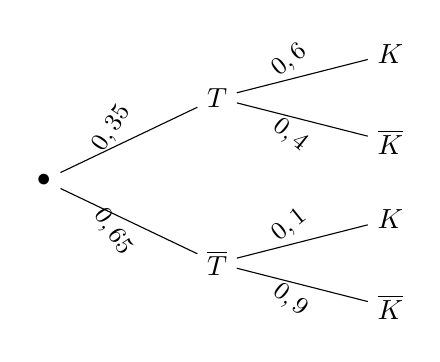
\begin{tikzpicture}[xscale=2.2,yscale=.7]
      \node (O) at (0,0) {$\bullet$};
      \node (T) at (1,1.5) {$T$}; \node (Tb) at (1,-1.5) {$\overline{T}$};
      \node (TK) at (2,2.3) {$K$}; \node (TKb) at (2,0.7) {$\overline{K}$};
      \node (TbK) at (2,-0.7) {$K$}; \node (TbKb) at (2,-2.3) {$\overline{K}$};
      \draw (O) -- node[above,sloped]{\small $0,35$} (T); \draw (O) -- node[below,sloped]{\small $0,65$} (Tb);
      \draw (T) -- node[above,sloped]{\small $0,6$} (TK); \draw (T) -- node[below,sloped]{\small $0,4$} (TKb);
      \draw (Tb) -- node[above,sloped]{\small $0,1$} (TbK); \draw (Tb) -- node[below,sloped]{\small $0,9$} (TbKb);
      \end{tikzpicture}
      \end{center}
\item $P(T\cap K) = P(T)\,P_T(K) = 0,35\times 0,6 = 0,21$. D'apr\`es la formule des probabilit\'es totales ($T$, $\overline{T}$ forment une partition) :
      $P(K) = P(T\cap K) + P(\overline{T}\cap K) = 0,21 + 0,65\times 0,1 = 0,21 + 0,065 = 0,275$.
\item $P(T)\,P(K) = 0,35\times 0,275 = 0,096\,25 \neq 0,21 = P(T\cap K)$ : $T$ et $K$ ne sont pas ind\'ependants
      (acheter un t\'el\'ephone rend l'achat d'une coque plus probable : $P_T(K) = 0,6 > P(K)$).
\item $P_K(T) = \dfrac{P(T\cap K)}{P(K)} = \dfrac{0,21}{0,275} = \dfrac{42}{55}\approx 0,764$.
\item $P_K(T) = \frac{42}{55}$, $P_K(\overline{T}) = \frac{0,065}{0,275} = \frac{13}{55}\approx 0,236$ ;
      $P(\overline{K}) = 0,725$, $P(T\cap\overline{K}) = 0,35\times 0,4 = 0,14$, donc
      $P_{\overline{K}}(T) = \frac{0,14}{0,725} = \frac{28}{145}\approx 0,193$ et
      $P_{\overline{K}}(\overline{T}) = \frac{0,585}{0,725} = \frac{117}{145}\approx 0,807$.
\end{enumerate}
\end{sol}
%
\begin{sol} (Exercice \ref{exo:proba-15}.)
\begin{enumerate}
\item Les deux pi\`eces sont ind\'ependantes : $P(B_1) = \frac{1}{2}\times\frac{1}{2} = \frac{1}{4}$, et $P(B_2) = \frac{3}{4}$.
\item Notons $W$ << le joueur gagne >>. $P_{B_1}(W) = \frac{4}{5}$ et $P_{B_2}(W) = \frac{1}{6}$. Par la formule des probabilit\'es totales :
      \[
      P(W) = \frac{1}{4}\times\frac{4}{5} + \frac{3}{4}\times\frac{1}{6} = \frac{1}{5} + \frac{1}{8} = \frac{13}{40}.
      \]
\item $P_W(B_1) = \dfrac{P(B_1\cap W)}{P(W)} = \dfrac{1/5}{13/40} = \dfrac{8}{13}\approx 0,615$.
      On passe de $\frac{1}{4}$ \`a $\frac{8}{13}$ : savoir que le joueur a gagn\'e rend beaucoup plus probable qu'il ait tir\'e dans $B_1$,
      la bo\^ite la plus riche en billets gagnants.
\item Les deux parties sont ind\'ependantes et chacune est perdue avec la probabilit\'e $\frac{27}{40}$ :
      $P(\text{au moins un gain}) = 1 - \left(\frac{27}{40}\right)^2 = 1 - \frac{729}{1\,600} = \frac{871}{1\,600}\approx 0,544$.
\end{enumerate}
\end{sol}
%
\begin{sol} (Exercice \ref{exo:proba-16}.)
\begin{enumerate}
\item $P(N) = 0,6$ ; $P_N(M) = \frac{1}{20} = 0,05$ ; $P_M(N) = \frac{1}{3}$.
\item $P(M\cap N) = P(N)\,P_N(M) = 0,6\times 0,05 = 0,03$. Comme $P_M(N) = \frac{P(M\cap N)}{P(M)}$,
      $P(M) = \dfrac{P(M\cap N)}{P_M(N)} = \dfrac{0,03}{1/3} = 0,09$.
\item $P(M\cap\overline{N}) = P(M) - P(M\cap N) = 0,06$ et $P(\overline{N}) = 0,4$, donc
      $P_{\overline{N}}(M) = \frac{0,06}{0,4} = 0,15$.
\item $P(M)\,P(N) = 0,09\times 0,6 = 0,054 \neq 0,03 = P(M\cap N)$ : $M$ et $N$ ne sont pas ind\'ependants.
      Le risque est de $5~\%$ avec moustiquaire et de $15~\%$ sans : dormir sous une moustiquaire divise ici le risque par $3$.
\end{enumerate}
\end{sol}
%
\begin{sol} (Exercice \ref{exo:proba-17}.)
\begin{enumerate}
\item Il y a $\C{n+4}{2} = \frac{(n+4)(n+3)}{2}$ paires \'equiprobables ; les paires gagnantes sont form\'ees d'un blanc et d'un noir : $n\times 4$.
      $p_n = \dfrac{4n}{(n+4)(n+3)/2} = \dfrac{8n}{(n+3)(n+4)}$.
\item $p_n = \dfrac{8n}{n^2 + 7n + 12} = \dfrac{8/n}{1 + 7/n + 12/n^2} \to 0$.
      C'\'etait pr\'evisible : quand $n$ est tr\`es grand, presque tous les jetons sont blancs et l'on tire presque toujours deux blancs.
\item $f'(x) = \dfrac{8(x+3)(x+4) - 8x(2x+7)}{(x+3)^2(x+4)^2} = \dfrac{8(12 - x^2)}{(x+3)^2(x+4)^2}$.
      $f$ est croissante sur $[1 ; 2\sqrt{3}]$ et d\'ecroissante sur $[2\sqrt{3} ; +\infty[$ ($2\sqrt{3}\approx 3,46$).
      Pour les entiers, le maximum est donc atteint en $n=3$ ou $n=4$ : $p_3 = \frac{24}{42} = \frac{4}{7}$ et $p_4 = \frac{32}{56} = \frac{4}{7}$.
      $p_n$ est maximale pour $n = 3$ et pour $n = 4$, et ce maximum vaut $\frac{4}{7}$.
\item \begin{enumerate}
      \item Chaque partie est une \'epreuve de Bernoulli (succ\`es : gagner, probabilit\'e $p_4 = \frac{4}{7}$) ;
            la remise des jetons rend les $5$ parties identiques et ind\'ependantes. $X$ suit la loi binomiale $B\!\left(5 ; \frac{4}{7}\right)$.
      \item $P(X=2) = \C{5}{2}\left(\frac{4}{7}\right)^2\left(\frac{3}{7}\right)^3 = \frac{10\times 16\times 27}{16\,807} = \frac{4\,320}{16\,807}\approx 0,257$.
      \item $P(X\geq 1) = 1 - P(X=0) = 1 - \left(\frac{3}{7}\right)^5 = \frac{16\,564}{16\,807}\approx 0,986$.
      \end{enumerate}
\end{enumerate}
\end{sol}
%
\begin{sol} (Exercice \ref{exo:proba-18}.)
\begin{description}
\item[A.] $60$ billets, dont $20$ gagnants et $40$ perdants.
      \begin{enumerate}
      \item Les paires de billets sont \'equiprobables ; le contraire de << au moins un gagnant >> est << deux perdants >> :
            $P = 1 - \dfrac{\C{40}{2}}{\C{60}{2}} = 1 - \dfrac{780}{1\,770} = 1 - \dfrac{26}{59} = \dfrac{33}{59}\approx 0,559$.
      \item Chaque jour, il n'a aucun gagnant avec la probabilit\'e $\frac{26}{59}$ ; les jours sont ind\'ependants :
            $P = 1 - \left(\frac{26}{59}\right)^3 \approx 0,914$.
      \item $P = 1 - \dfrac{\C{40}{4}}{\C{60}{4}} = 1 - \dfrac{91\,390}{487\,635} = \dfrac{4\,171}{5\,133}\approx 0,813$.
            Deux billets deux jours de suite donnent $1 - \left(\frac{26}{59}\right)^2 = \frac{2\,805}{3\,481}\approx 0,806$ :
            acheter quatre billets le m\^eme jour est (un peu) plus avantageux.
      \end{enumerate}
\item[B.] \begin{enumerate}
      \item Il y a $2n$ billets perdants :
            $u_n = 1 - \dfrac{\C{2n}{2}}{\C{3n}{2}} = 1 - \dfrac{2n(2n-1)}{3n(3n-1)} = 1 - \dfrac{2(2n-1)}{3(3n-1)} = \dfrac{9n - 3 - 4n + 2}{3(3n-1)} = \dfrac{5n-1}{3(3n-1)}$.
            (Pour $n = 20$ on retrouve $\frac{99}{177} = \frac{33}{59}$.)
      \item $u_{n+1} - u_n = \dfrac{5n+4}{3(3n+2)} - \dfrac{5n-1}{3(3n-1)} = \dfrac{(5n+4)(3n-1) - (5n-1)(3n+2)}{3(3n+2)(3n-1)} = \dfrac{-2}{3(3n+2)(3n-1)} < 0$.
            La suite $(u_n)$ est strictement d\'ecroissante ($u_1 = \frac{2}{3}$).
            $u_n = \dfrac{5 - 1/n}{3(3 - 1/n)} \to \dfrac{5}{9}$.
      \item Avec remise, chaque billet est perdant avec la probabilit\'e $\frac{2}{3}$, et
            $P(\text{au moins un gagnant}) = 1 - \left(\frac{2}{3}\right)^2 = \frac{5}{9}$.
            Quand le nombre de billets est tr\`es grand, retirer un billet ne change presque pas la composition :
            le tirage sans remise se comporte comme un tirage avec remise.
      \end{enumerate}
\end{description}
\end{sol}
%
\begin{sol} (Exercice \ref{exo:proba-19}.)
\begin{enumerate}
\item $X$ prend les valeurs $0$, $1$, $2$, $3$, $4$. Les $4$ lancers sont des \'epreuves de Bernoulli identiques (succ\`es : r\'eussir, $p = 0,7$) et ind\'ependantes :
      $X$ suit la loi binomiale $B(4 ; 0,7)$, et $P(X=k) = \C{4}{k}\,0,7^k\,0,3^{4-k}$.
\item \[
      \begin{array}{|c|c|c|c|c|c|}
      \hline
      k & 0 & 1 & 2 & 3 & 4 \\ \hline
      P(X=k) & 0,008\,1 & 0,075\,6 & 0,264\,6 & 0,411\,6 & 0,240\,1 \\ \hline
      \end{array}
      \]
      $0,008\,1 + 0,075\,6 + 0,264\,6 + 0,411\,6 + 0,240\,1 = 1$.
\item $P(X\geq 2) = 1 - P(X=0) - P(X=1) = 1 - 0,083\,7 = 0,916\,3$.
\item $F(x) = 0$ si $x < 0$ ; $F(x) = 0,008\,1$ si $0\le x<1$ ; $F(x) = 0,083\,7$ si $1\le x<2$ ;
      $F(x) = 0,348\,3$ si $2\le x<3$ ; $F(x) = 0,759\,9$ si $3\le x<4$ ; $F(x) = 1$ si $x\geq 4$.
      La courbe est en escalier, croissante, avec des sauts en $0$, $1$, $2$, $3$, $4$ (comme dans l'exemple du cours).
\item $E[X] = 0,075\,6 + 2\times 0,264\,6 + 3\times 0,411\,6 + 4\times 0,240\,1 = 2,8$ ;
      $E[X^2] = 0,075\,6 + 4\times 0,264\,6 + 9\times 0,411\,6 + 16\times 0,240\,1 = 8,68$, donc
      $V(X) = 8,68 - 2,8^2 = 0,84$ et $\sigma(X) = \sqrt{0,84}\approx 0,917$.
      Formules : $np = 4\times 0,7 = 2,8$ et $np(1-p) = 4\times 0,7\times 0,3 = 0,84$.
\end{enumerate}
\end{sol}
%
\begin{sol} (Exercice \ref{exo:proba-20}.)
\begin{enumerate}
\item Chaque roue a $6$ secteurs de m\^eme taille : $6^3 = 216$ r\'esultats, \'equiprobables (roues ind\'ependantes).
\item \begin{enumerate}
      \item Trois \'etoiles : $1^3 = 1$ cas ; trois lunes : $2^3 = 8$ ; trois soleils : $3^3 = 27$.
            $P = \frac{36}{216} = \frac{1}{6}$.
      \item Contraire : aucune \'etoile, $5^3 = 125$ cas. $P = 1 - \frac{125}{216} = \frac{91}{216}$.
      \item Position de la lune : $3$ choix ; puis $1\times 1\times 2$ secteurs. $\frac{3\times 2}{216} = \frac{1}{36}$.
      \end{enumerate}
\item \begin{enumerate}
      \item Trois \'etoiles : $\frac{1}{216}$. Exactement deux \'etoiles : position de la roue sans \'etoile ($3$ choix) et $5$ secteurs pour elle :
            $\frac{15}{216} = \frac{5}{72}$. Sinon : $\frac{200}{216} = \frac{25}{27}$.
            \[
            \begin{array}{|c|c|c|c|}
            \hline
            g & 9\,900 & 900 & -100 \\ \hline
            P(G = g) & \frac{1}{216} & \frac{15}{216} & \frac{200}{216} \\ \hline
            \end{array}
            \]
      \item $E[G] = \dfrac{9\,900 + 15\times 900 - 200\times 100}{216} = \dfrac{3\,400}{216} = \dfrac{425}{27}\approx 15,74$~Ar.
            L'esp\'erance est positive : le jeu est favorable au joueur (en moyenne il gagne environ $15,74$~Ar par partie).
      \item Si la partie co\^ute $m$ ariary, $E[G] = \frac{10\,000 + 15\times 1\,000}{216} - m = \frac{3\,125}{27} - m$.
            Le jeu est \'equitable pour $m = \frac{3\,125}{27}\approx 115,74$~Ar.
      \end{enumerate}
\item Il faudrait (somme)$\times$(probabilit\'e) constant. Or $10\,000\times\frac{1}{216} \neq 1\,000\times\frac{15}{216}$ :
      le principe n'est pas respect\'e. Pour le respecter, il faudrait verser $s$ avec $s\times 15 = 10\,000\times 1$,
      soit $s = \frac{2\,000}{3}\approx 667$~Ar pour exactement deux \'etoiles.
\end{enumerate}
\end{sol}
%
\begin{sol} (Exercice \ref{exo:proba-21}.)
\begin{enumerate}
\item Quatre choix pour chacune des six questions : $4^6 = 4\,096$ copies.
\item \begin{enumerate}
      \item Chaque question est une \'epreuve de Bernoulli (succ\`es : r\'eponse exacte, $p = \frac{1}{4}$),
            les r\'eponses au hasard sont ind\'ependantes : $X$ suit $B\!\left(6 ; \frac{1}{4}\right)$.
      \item $P(X=0) = \left(\frac{3}{4}\right)^6 = \frac{729}{4\,096}\approx 0,178$ ;
            $P(X=2) = \C{6}{2}\left(\frac{1}{4}\right)^2\left(\frac{3}{4}\right)^4 = \frac{15\times 81}{4\,096} = \frac{1\,215}{4\,096}\approx 0,297$ ;
            $P(X\geq 3) = P(X=3)+\cdots+P(X=6) = \frac{540 + 135 + 18 + 1}{4\,096} = \frac{694}{4\,096} = \frac{347}{2\,048}\approx 0,169$.
      \item Les copies sym\'etriques sont d\'etermin\'ees par leurs trois premi\`eres lettres : $4^3 = 64$ copies.
            Les copies sont \'equiprobables, donc $P = \frac{64}{4\,096} = \frac{1}{64}$.
      \end{enumerate}
\item \begin{enumerate}
      \item $S = 3X - (6 - X) = 4X - 6$.
      \item $E[S] = \sum_k (4k-6)\,P(X=k) = 4\sum_k k\,P(X=k) - 6\sum_k P(X=k) = 4E[X] - 6 = 4\times\frac{6}{4} - 6 = 0$.
            $V(S) = E\big[(S - 0)^2\big] = E\big[(4X - 6)^2\big] = 16\,E\big[(X - \tfrac{3}{2})^2\big] = 16\,V(X) = 16\times 6\times\frac{1}{4}\times\frac{3}{4} = 18$.
            En r\'epondant au hasard, un candidat obtient en moyenne $0$ point : le hasard ne rapporte rien en moyenne.
      \end{enumerate}
\item Pour chaque \'el\`eve, l'\'ev\`enement << aucune r\'eponse exacte >> a la probabilit\'e $r = \frac{729}{4\,096}$ ;
      les $32$ \'el\`eves r\'epondent ind\'ependamment : $Y$ suit $B(32 ; r)$.
      $P(Y\leq 1) = (1-r)^{32} + 32\,r\,(1-r)^{31}\approx 0,001\,9 + 0,013\,1 \approx 0,015$.
      $E[Y] = 32\times\frac{729}{4\,096} = \frac{729}{128}\approx 5,7$.
\end{enumerate}
\end{sol}
%
\begin{sol} (Exercice \ref{exo:proba-22}.)
\begin{enumerate}
\item \begin{enumerate}
      \item Par ind\'ependance, $P(A\cap B) = 0,04\times 0,05 = 0,002$.
      \item $P(A\cup B) = 0,04 + 0,05 - 0,002 = 0,088$.
      \item Premi\`ere m\'ethode : $P(\overline{A\cup B}) = 1 - 0,088 = 0,912$.
            Seconde m\'ethode : $\overline{A}$ et $\overline{B}$ sont aussi ind\'ependants, donc
            $P(\overline{A}\cap\overline{B}) = 0,96\times 0,95 = 0,912$.
      \item $P_A(B) = \frac{P(A\cap B)}{P(A)} = \frac{0,002}{0,04} = 0,05 = P(B)$, ce qui traduit l'ind\'ependance.
      \end{enumerate}
\item \begin{enumerate}
      \item $50$ \'epreuves de Bernoulli identiques et ind\'ependantes (succ\`es : pot d\'efectueux, $p = 0,088$) :
            $X$ suit $B(50 ; 0,088)$.
      \item $P(X=0) = 0,912^{50}\approx 0,010$ ; $P(X\geq 1) = 1 - 0,912^{50}\approx 0,990$.
      \item $P(X\leq 2) = 0,912^{50} + 50\times 0,088\times 0,912^{49} + \C{50}{2}\times 0,088^2\times 0,912^{48}\approx 0,172$.
      \item $E[X] = 50\times 0,088 = 4,4$ et $\sigma(X) = \sqrt{50\times 0,088\times 0,912} = \sqrt{4,012\,8}\approx 2,00$.
            Sur un grand nombre d'achats de $50$ pots, il y a en moyenne $4,4$ pots d\'efectueux par achat.
      \end{enumerate}
\end{enumerate}
\end{sol}
%
\begin{sol} (Exercice \ref{exo:proba-23}.)
\begin{enumerate}
\item $P(D) = 0,1$, $P(\overline{D}) = 0,9$ ; $P_D(R) = 0,95$, $P_D(\overline{R}) = 0,05$ ; $P_{\overline{D}}(R) = 0,04$, $P_{\overline{D}}(\overline{R}) = 0,96$
      (m\^eme forme d'arbre que dans l'Exercice~\ref{exo:proba-14}).
\item \begin{enumerate}
      \item $P(D\cap\overline{R}) = 0,1\times 0,05 = 0,005$.
      \item $P(\overline{D}\cap R) + P(D\cap\overline{R}) = 0,9\times 0,04 + 0,005 = 0,036 + 0,005 = 0,041$.
      \end{enumerate}
\item Probabilit\'es totales : $P(R) = 0,1\times 0,95 + 0,9\times 0,04 = 0,095 + 0,036 = 0,131$, donc $P(\overline{R}) = 0,869$ et
      $P_{\overline{R}}(D) = \dfrac{0,005}{0,869} = \dfrac{5}{869}\approx 0,005\,8$.
      Moins de $0,6~\%$ des gousses accept\'ees sont insuffisantes, contre $10~\%$ avant le tri.
\item \begin{enumerate}
      \item Le nombre $Y$ de rejets suit $B(3 ; 0,131)$. Gains : extra $6\,000 - 2\,000 = 4\,000$ ; standard $1\,000$ ; d\'etruite $-2\,000$.
            \[
            \begin{array}{|c|c|c|c|}
            \hline
            g & 4\,000 & 1\,000 & -2\,000 \\ \hline
            P(G=g) & 0,869^3\approx 0,656\,2 & 3\times 0,131\times 0,869^2\approx 0,296\,8 & 1 - P(Y\le 1)\approx 0,047\,0 \\ \hline
            \end{array}
            \]
      \item $E[G] = 4\,000\times 0,869^3 + 1\,000\times 3\times 0,131\times 0,869^2 - 2\,000\times P(Y\geq 2)\approx 2\,828$~Ar.
            Pour $10\,000$ gousses, la coop\'erative peut esp\'erer un b\'en\'efice d'environ $28$ millions d'ariary.
      \end{enumerate}
\end{enumerate}
\end{sol}
\end{corrige}
